\section{译者补充:经典电磁理论下的光学基础}\label{sec:译者补充:经典电磁理论下的光学基础}
\begin{remark}
    本节内容不是原书内容,而是译者根据\citet{hecht2016optics}、
    \citet{hass2023}、\citet{9780199573363}、\citet{978-0471021988}、\citet{enwiki:1320467269,enwiki:1307793858}
    补充并参考\citet{OpticsChinese}翻译的,请酌情参考和斧正。
    本节内容只简要介绍相关基础概念和结论,
    并不像正式的物理和光学教材那样严谨,请读者批判性地看待本节内容。
    本节要求读者具备较好的微积分与电磁理论知识储备。
    此外读者需注意,本节遵循有关内容惯例采用右手坐标系,
    与正文pbrt采用的左手坐标系不同。
\end{remark}

\subsection{波动}\label{sub:波动}
光的本质是什么?光是波动现象还是粒子现象?这个问题非常复杂。
然而当我们站在通常的大尺度视角下时,电磁波及其经典理论已经够用了。
为了打好基础,我们从波的数学描述说起,它也适用于一切物理波。

\subsubsection*{一维波}
行进中的\keyindex{波}{wave}{}
的一个本质特性是,它是传播波的\keyindex{介质}{medium}{}
的自持\keyindex{扰动}{disturbance}{}。
\keyindex{机械波}{mechanical wave}{wave\ 波}
是我们最熟悉的波,例如琴弦上的波、液体表面的波以及
空气中的\keyindex{声波}{sound wave}{wave\ 波}。
波还有纵波、横波之分。介质在波动方向上位移的是\keyindex{纵波}{longitudinal wave}{wave\ 波}。
介质位移的方向垂直于波动方向的是\keyindex{横波}{transverse wave}{wave\ 波}。
例如,声波是纵波;琴弦上的波、电磁波是横波。
波区别于粒子流的几个关键特征之一是,
扰动在前进,但实物介质并不前进。
就像风吹起滚滚麦浪,但麦穗只是原地摇摆。
\begin{figure}[htbp]
    \centering
    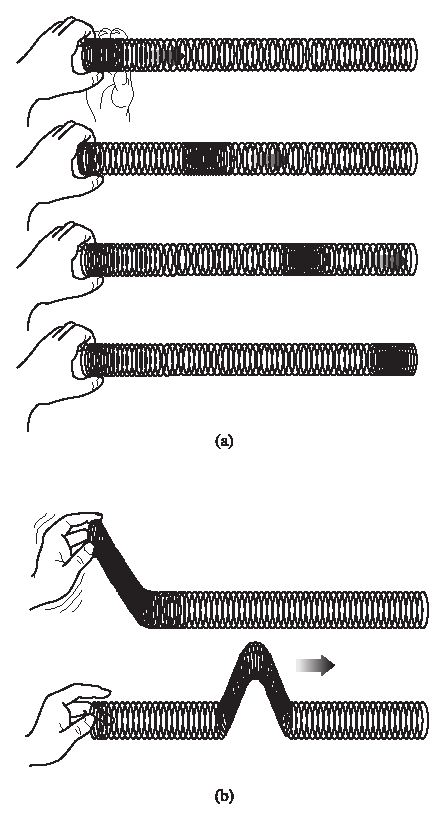
\includegraphics[width=0.65\linewidth]{Pictures/chap08/longitudinalAndTransverseWave.eps}
    \caption{弹簧中的(a)纵波;(b)横波。}
    \label{fig:08ex02.0201}
\end{figure}

我们暂不追究扰动的本质,而专注研究描述波动的方程应该具备怎样的形式。
设某个这样的扰动$\psi$以恒定速度$v$沿正$x$方向运动。
既然扰动在运动,则它必然是位置和时间的函数:
\begin{align}
    \psi(x,t)=f(x,t)\, ,
\end{align}
其中$f(x,t)$对应于某个具体函数或波形。
如\reffig{08ex02.0203}(a)所示,一个脉冲在静止坐标系$S$中以速度$v$运动。
我们取定任意时刻$t$即可得到那个时刻波的\keyindex{剖面}{profile}{},
就像脉冲经过时给它“拍照”。例如$t=0$有
\begin{align}
    \psi(x,t)\bigg|_{t=0}=f(x,0)=f(x)
\end{align}
表示0时刻波的剖面。
\begin{figure}[htb]
    \centering
    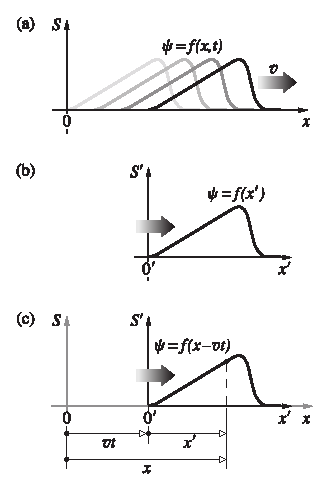
\includegraphics[width=0.5\linewidth]{Pictures/chap08/MovingReferenceFrame.eps}
    \caption{运动参考系。}
    \label{fig:08ex02.0203}
\end{figure}

现在,我们先只考虑传播时形状不变的波。
在一段时间$t$后,脉冲沿$x$轴前进了距离$vt$,其余不变。
如\reffig{08ex02.0203}(b),我们引入新坐标系$S'$并与脉冲以相同速度$v$运动。
则在该坐标系中$\psi$不再是时间的函数,而是静止不变的剖面,即
\begin{align}
    \psi=f(x')\, ,
\end{align}
这意味着坐标系$S'$中的扰动在任意时刻$t$的形状,
都和$S$中$t=0$时两者具有同一原点时扰动的形状相同,如\reffig{08ex02.0203}(c)所示。
为了将上式改写为$S$中某静止观察者描述的形式,我们利用
\begin{align}
    x'=x-vt
\end{align}
得到
\begin{align}
    \psi(x,t)=f(x-vt)\, .
\end{align}
上式是一维\keyindex{波函数}{wave function}{wave\ 波}
的最一般形式。它描述了一个具有所需剖面形状$f(x)$的波,它以速度$v>0$沿正$x$方向运动。
相似地,如果波向负$x$方向运动,则上式应改写为
\begin{align}
    \psi(x,t)=f(x+vt)\, .
\end{align}
总之变量$x$和$t$一定作为一个整体变量$x\mp vt$出现。

\subsubsection*{波动微分方程}
接下来我们推导一维波动方程的形式,把$\psi(x,t)$对空间与时间的依赖关系联系起来。注意到
\begin{align}
    \frac{\partial x'}{\partial x}=\frac{\partial (x\mp vt)}{\partial x}=1\, ,
\end{align}
以及
\begin{align}
    \frac{\partial x'}{\partial t}=\mp v\, ,
\end{align}
所以$\psi(x,t)$在$t$恒定时对$x$的偏微分为
\begin{align}
    \frac{\partial \psi}{\partial x}
    =\frac{\partial f}{\partial x}
    =\frac{\partial f}{\partial x'}\frac{\partial x'}{\partial x}
    =\frac{\partial f}{\partial x'}\, .
\end{align}
而在$x$恒定时$\psi(x,t)$对$t$的偏微分为
\begin{align}
    \frac{\partial \psi}{\partial t}
    =\frac{\partial f}{\partial t}
    =\frac{\partial f}{\partial x'}\frac{\partial x'}{\partial t}
    =\mp v\frac{\partial f}{\partial x'}
    =\mp v\frac{\partial \psi}{\partial x}\, .
\end{align}
上式表明$\psi$对$x$和$t$的变化率只差一个常系数。
继续求$\psi$的二阶偏微分有
\begin{align}
    \frac{\partial^2 \psi}{\partial x^2}
    =\frac{\partial}{\partial x}\left(\frac{\partial \psi}{\partial x}\right)
    =\frac{\partial}{\partial x}\left(\frac{\partial f}{\partial x'}\right)
    =\frac{\partial}{\partial x'}\left(\frac{\partial f}{\partial x'}\right)\frac{\partial x'}{\partial x}
    =\frac{\partial^2 f}{\partial x'^2}\, ,
\end{align}
并进一步得到
\begin{align}
    \frac{\partial^2 \psi}{\partial t^2}
    = & \frac{\partial}{\partial t}\left(\frac{\partial \psi}{\partial t}\right)
    =\frac{\partial}{\partial t}\left(\mp v\frac{\partial f}{\partial x'}\right)\nonumber    \\
    = & \mp v\frac{\partial}{\partial x'}\left(\frac{\partial f}{\partial t}\right)
    =\mp v\frac{\partial}{\partial x'}\left(\frac{\partial \psi}{\partial t}\right)\nonumber \\
    = & \mp v\frac{\partial}{\partial x'}\left(\mp v\frac{\partial f}{\partial x'}\right)
    =v^2\frac{\partial^2 f}{\partial x'^2}\nonumber                                          \\
    = & v^2\frac{\partial^2 \psi}{\partial x^2}\, .
\end{align}
整理上式即
\begin{definition}[一维\keyindex{波动微分方程}{differential wave equation}{equation\ 方程}]
    \begin{align}
        \frac{\partial^2 \psi}{\partial x^2}=\frac{1}{v^2}\frac{\partial^2 \psi}{\partial t^2}\, .
    \end{align}
\end{definition}
注意上式是一个\keyindex{齐次微分方程}{homogeneous differential equation}{equation\ 方程},
没有仅含独立变量的项(例如一份“力”或“源”),
所以描述的是\keyindex{无阻尼系统}{undamped system}{system\ 系统}。
这意味着若$\psi$是方程的解,则它乘以任意倍数后也是解。
反之,若一个波函数是上述方程的解,则它将是$x\mp vt$的函数,
且可以对$x$和$t$求得非平凡的二阶微分。

\subsubsection*{谐波}
最简单的波形是正弦或余弦曲线。它可以称作
\keyindex{正弦波}{sinusoidal wave}{wave\ 波}、
\keyindex{简谐波}{simple harmonic wave}{wave\ 波}
或\keyindex{谐波}{harmonic wave}{wave\ 波}。
任何波形都可以由谐波叠加合成。

我们为谐波波形选定为以下简单函数:
\begin{align}
    \psi(x,t)\bigg|_{t=0}=\psi(x)=f(x)=A\sin kx\, ,
\end{align}
其中常数$k>0$称作\keyindex{传播数}{propagation number}{},
$kx$这个整体是无量纲的。$\psi(x)$的最大值$A>0$称作波的\keyindex{振幅}{amplitude}{}。
将上式中的$x$替换为$x-vt$,改写成以速度$v$沿正$x$方向前进的波:
\begin{align}
    \psi(x,t)=A\sin k(x-vt) = f(x-vt)\, .
\end{align}
显然它是波动微分方程的一个解。该波在空间和时间中都具有周期性。
它的\keyindex{空间周期}{spatial period}{period\ 周期}
称作\keyindex{波长}{wavelength}{},表示每个波的长度,记作$\lambda$.
当$x$大小增减$\lambda$,$\psi$应不变:
\begin{align}
    \psi(x,t)=\psi(x\pm\lambda,t)\, .
\end{align}
这对应了正弦函数自变量改变$\pm2\pi$,由于$k>0,\ \lambda>0$,所以
\begin{align}
    \lambda=\frac{2\pi}{k}\, .
\end{align}

类似地,$\psi$的\keyindex{时间周期}{temporal period}{period\ 周期}记作$\tau$,
可简称\keyindex{周期}{period}{},即一个完整的波经过一静止观察者的时间。
它对应了波在时间上的重复行为:
\begin{align}
    \psi(x,t)=\psi(x,t\pm\tau)\, .
\end{align}
由此我们容易推出
\begin{align}
    kv\tau=2\pi\, ,
\end{align}
以及
\begin{align}
    \tau=\frac{\lambda}{v}\, .
\end{align}

周期的倒数称作\keyindex{时间频率}{temporal frequency}{frequency\ 频率},
可简称\keyindex{频率}{frequency}{},记作$\nu$,即单位时间里波的个数:
\begin{align}
    \nu=\frac{1}{\tau}\, ,
\end{align}
其单位为\keyindex{赫兹}{Hertz}{}
(Hz)\begin{marginfigure}
    \includegraphics[width=\linewidth]{chap08/HEINRICH_HERTZ.jpg}
\end{marginfigure}\sidenote{德国物理学家海因里希·鲁道夫·赫兹 (Heinrich Rudolf Hertz, 1857-1894)。},
即每秒周数。结合前述定义,不难发现\keyindex{波速}{speed}{}
$v$满足\sidenote{注意$v$是英语字母,$\nu$是希腊字母。}
\begin{align}
    v=\nu\lambda\, .
\end{align}

此外我们还定义\keyindex{时间角频率}{angular temporal frequency}{frequency\ 频率}
为
\begin{align}
    \omega=\frac{2\pi}{\tau}=2\pi\nu=kv\, ,
\end{align}
可简称为\keyindex{角频率}{angular frequency}{frequency\ 频率},单位为弧度每秒(rad/s)。

此外,\keyindex{空间频率}{spatial frequency}{frequency\ 频率},
也称\keyindex{波数}{wavenumber}{},定义为
\begin{align}
    \kappa=\frac{1}{\lambda}\, ,
\end{align}
即单位长度中波的数目,单位为$\mathrm{m}^{-1}$.

以上所有概念也适用于非谐波,只要它是由单个剖面元规则重复构成的。

利用以上定义,我们可以写出以下常见而等价的谐波表达式:
\begin{align}
    \psi= & A\sin k(x\mp vt)\, ,                                                                           \\
    \psi= & A\sin (kx\mp\omega t)\, ,                                                                      \\
    \psi= & A\sin 2\pi\left(\frac{x}{\lambda}\mp\frac{t}{\tau}\right)\, , \label{eq:08ex02-HarmonicWave03} \\
    \psi= & A\sin 2\pi(\kappa x\mp\nu t)\, ,                                                               \\
    \psi= & A\sin 2\pi\nu\left(\frac{x}{v}\mp t\right)\, ,
\end{align}
其中前两个最为常用,你甚至可以改用余弦函数来表示(后文就有)。
注意到这些理想化波的$x$和$t$没有取值范围限制,
又具有单一恒定频率,所以称作是\keyindex{单色的}{monochromatic}{}
或\keyindex{单能量的}{monoenergetic}{}。
但真实的波无法无限回溯到$t=-\infty$,所以不会是严格的单色波,而是含有一个频率范围。
若这个频段很窄,则称该波是\keyindex{准单色的}{quasimonochromatic}{}。

\begin{example}
    以国际单位制下的如下函数为例:
    \begin{align}
        \psi(y,t)=0.040\times\sin 2\pi\left(\frac{y}{6.0\times10^{-7}}+\frac{t}{2.0\times10^{-15}}\right)\, .
    \end{align}
    它与\refeq{08ex02-HarmonicWave03}形式一致,所以表示的是谐波,沿着$y$的负方向传播。其周期为
    \begin{align}
        \tau=2.0\times10^{-15}\text{s}\, .
    \end{align}
    频率为
    \begin{align}
        \nu=\frac{1}{\tau}=5.0\times10^{14}\text{Hz}\, .
    \end{align}
    波长为
    \begin{align}
        \lambda=6.0\times10^{-7}\text{m}\, .
    \end{align}
    振幅为
    \begin{align}
        A=0.040\, .
    \end{align}
    速度为
    \begin{align}
        v=\nu\lambda=(5.0\times10^{14})\times(6.0\times10^{-7})=3.0\times10^8\text{m/s}\, .
    \end{align}
\end{example}

\subsubsection*{相位与相速度}
考察任一谐波,如
\begin{align}
    \psi(x,t)= & A\sin (kx-\omega t)\, ,
\end{align}
称正弦函数的整个输入值为波的\keyindex{相位}{phase}{},记作
\begin{align}
    \varphi=kx-\omega t\, .
\end{align}
更普遍地,对于谐波
\begin{align}
    \psi(x,t)= & A\sin (kx-\omega t+\varepsilon)\, ,
\end{align}
其相位为
\begin{align}
    \varphi=kx-\omega t+\varepsilon\, ,
\end{align}
其中$t=0$且$x=0$时的相位$\varepsilon$称作\keyindex{初相}{initial phase}{}。

根据相位定义,可知当$x$恒定时,相位对时间的变化率为
\begin{align}
    \left|\left(\frac{\partial\varphi}{\partial t}\right)_x\right|=\omega\, .
\end{align}
当$t$恒定时,相位对距离的变化率为
\begin{align}
    \left|\left(\frac{\partial\varphi}{\partial x}\right)_t\right|=k\, .
\end{align}
利用链式法则等微分知识,可推得
\begin{align}
    \left(\frac{\partial x}{\partial t}\right)_{\varphi}
    =-\displaystyle\frac{(\partial\varphi/\partial t)_x}
    {(\partial\varphi/\partial x)_t}
    =\pm\frac{\omega}{k}=\pm v\, .
\end{align}
上式最左边表示相位恒定状态的传播速度,称作波的\keyindex{相速度}{phase velocity}{}。
这里$v>0$,当波朝着正$x$方向运动时,则相速度取正号,反之则取负号。

\subsubsection*{叠加原理}
波动微分方程揭示了波一个明显区别于经典粒子流的性质:
\begin{theorem}[\keyindex{叠加原理}{superposition principle}{}]
    若$\psi_1$和$\psi_2$是同一波动方程的两个不同的解,
    则叠加它们的$\psi_1+\psi_2$也是一个解。
\end{theorem}
这意味着两个波到达同一片空间时会发生重叠,
简单地与另一方相加(相减),而不会永久瓦解其中某个波。
重叠区域内每一点的合扰动是该位置上单个成分波的代数之和。
在穿过共存区域后,每个波会继续前进离开,不受这次干扰。
注意这里我们讨论的是最为广泛的波的线性叠加,
暂不考虑极端情况下波的振幅大到以非线性方式驱动介质。

\begin{figure}[htb]
    \centering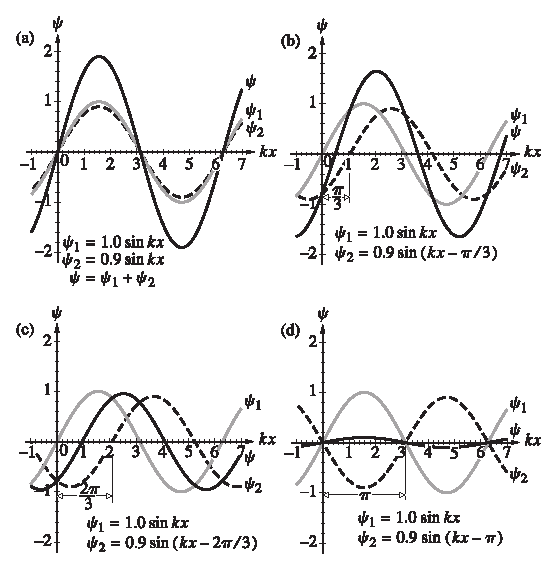
\includegraphics[width=0.9\linewidth]{Pictures/chap08/SuperpositionOfTwoSinusoids.eps}
    \caption{两个正弦波$\psi_1$和$\psi_2$的叠加,振幅分别为$A_1=1.0$和$A_2=0.9$.
        (a)$\psi_1$和$\psi_2$同相。(b)$\psi_1$领先$\psi_2$相角$\displaystyle\frac{\pi}{3}$.
        (c)$\psi_1$领先$\psi_2$相角$\displaystyle\frac{2\pi}{3}$.
        (d)$\psi_1$和$\psi_2$相位相差$\pi$,几乎要相互抵消。}
    \label{fig:08ex02.0216}
\end{figure}
\reffig{08ex02.0216}展示了两个振幅十分接近的波叠加后的结果与它们之间相位差的关系。
\reffig{08ex02.0216}(a)中两个波相位差为零,称为\keyindex{同相}{in-phase}{}。
它们互相加强,振幅增大,频率和波长不变。随着相位差增大,合成波振幅减小,
直到\reffig{08ex02.0216}(d)中相位差达到$\pi$,合成波几乎消失,
此时称两个波\keyindex{异相}{out-of-phase}{}
$180^\circ$.
异相波倾向于互相抵消的现象使得这整类现象被称作\keyindex{干涉}{interference}{}。

\subsubsection*{波的复数表示}
谐波所含的三角函数不便于数学处理,因此我们引入更方便的复数表示方法
\sidenote{本节复数等数学符号暂时遵循参考文献的记法。}。
\keyindex{复数}{complex number}{}
$\widetilde{z}$形如
\begin{align}
    \widetilde{z}=x+\mathrm{i}y=r(\cos\theta+\mathrm{i}\sin\theta)=r\mathrm{e}^{\mathrm{i}\theta}\, ,
\end{align}
其中\keyindex{虚数单位}{imaginary unit}{}
$\mathrm{i}=\sqrt{-1}$.
实数$x$和$y$分别为$\widetilde{z}$的\keyindex{实部}{real part}{complex number\ 复数}
和\keyindex{虚部}{imaginary part}{complex number\ 复数};
实数$r\ge0$和$\theta$分别为$\widetilde{z}$的\keyindex{长度}{magnitude}{complex number\ 复数}
和\keyindex{相角}{phase angle}{complex number\ 复数};
长度也常记作$|\widetilde{z}|$,称为复数的\keyindex{模}{modulus}{complex number\ 复数}
或\keyindex{绝对值}{absolute value}{complex number\ 复数}。

本节中,复数的\keyindex{复共轭}{complex conjugate}{}
用星号表示,即
\begin{align}
    \widetilde{z}^*=(x+\mathrm{i}y)^*=x-\mathrm{i}y
    =r(\cos\theta-\mathrm{i}\sin\theta)=r\mathrm{e}^{-\mathrm{i}\theta}\, .
\end{align}
于是复数的实部和虚部可以表示为
\begin{align}
    \mathrm{Re}(\widetilde{z}) & =\frac{1}{2}(\widetilde{z}+\widetilde{z}^*)=r\cos\theta\, ,           \\
    \mathrm{Im}(\widetilde{z}) & =\frac{1}{2\mathrm{i}}(\widetilde{z}-\widetilde{z}^*)=r\sin\theta\, .
\end{align}
我们习惯上选用实部来描述谐波,即
\begin{align}
    \psi(x,t)=\mathrm{Re}[A\mathrm{e}^{\mathrm{i}(\omega t-kx+\varepsilon)}]\, ,
\end{align}
它等价于
\begin{align}
    \psi(x,t)=A\cos(\omega t-kx+\varepsilon)\, .
\end{align}
于是为了方便,在后文中我们略去实部记号把波函数简写为
\begin{align}
    \psi(x,t)=A\mathrm{e}^{\mathrm{i}(\omega t-kx+\varepsilon)}=A\mathrm{e}^{\mathrm{i}\varphi}\, ,
\end{align}
并借助复数运算法则(尤其是复指数乘除法的简便性)来进行计算,
只在要表示实际波时才取回实部。

要注意的是,波被表示为复数函数后,若参与了运算,
则只有当这些运算仅限于加减法、乘或除以一个实数,
或对一个实数变量进行微分或积分,才能恢复其实部,否则结果是错误的。

\subsubsection*{平面波}
给定时刻的光波可以用其频率、振幅、传播方向等描述,
但这并没有告诉我们光扰动在一片延伸的空间内的更多信息。
为此我们已经在定义\ref{definition:wavefront}中
引入了\keyindex{波阵面}{wavefront}{}
的概念。本节将研究理想的平面波的数学表达
\sidenote{本节向量等数学符号暂时遵循参考文献的记法。}。

\begin{figure}[htbp]
    \centering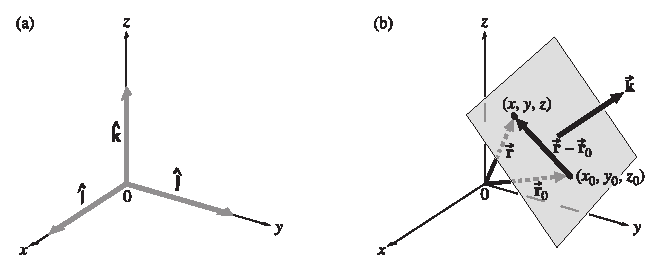
\includegraphics[width=\linewidth]{Pictures/chap08/CartesianUnitBasisVectors.eps}
    \caption{(a)直角坐标系单位基向量。(b)沿着$\vec{\mathbf{k}}$方向运动的平面波。}
    \label{fig:08ex02.0221}
\end{figure}
\keyindex{平面波}{plane wave}{wave\ 波}
是最简单的三维波了,其扰动的一切等相面构成一组平面,
且一般都垂直于传播方向。为此我们先给出平面的数学表达式:
如\reffig{08ex02.0221}(a)所示,对于直角坐标系中
的位置向量$\vec{\mathbf{r}}$,我们用三个坐标轴上的单位基向量来表示为
\begin{align}
    \vec{\mathbf{r}}=x\hat{\text{\sffamily\bfseries i}}+y\hat{\text{\sffamily\bfseries j}}+z\hat{\text{\sffamily\bfseries k}}\, .
\end{align}
它始于某个任意的原点$O$,止于点$(x,y,z)$,该点可以是空间中的任意位置。
类似地如\reffig{08ex02.0221}(b)所示,有
\begin{align}
    \vec{\mathbf{r}}-\vec{\mathbf{r}}_0
    =(x-x_0)\hat{\text{\sffamily\bfseries i}}+(y-y_0)\hat{\text{\sffamily\bfseries j}}+(z-z_0)\hat{\text{\sffamily\bfseries k}}\, .
\end{align}
我们令
\begin{align}
    (\vec{\mathbf{r}}-\vec{\mathbf{r}}_0)\cdot\vec{\mathbf{k}}=0\, ,
\end{align}
使向量$\vec{\mathbf{r}}-\vec{\mathbf{r}}_0$扫过
一垂直于$\vec{\mathbf{k}}$的平面,其端点$(x,y,z)$取一切允许的值。
设$\vec{\mathbf{k}}$为
\begin{align}
    \vec{\mathbf{k}}=k_x\hat{\text{\sffamily\bfseries i}}+k_y\hat{\text{\sffamily\bfseries j}}+k_z\hat{\text{\sffamily\bfseries k}}\, ,
\end{align}
则有
\begin{align}
    k_x(x-x_0)+k_y(y-y_0)+k_z(z-z_0)=0\, ,
\end{align}
即
\begin{align}
    k_xx+k_yy+k_zz=a\, ,
\end{align}
其中
\begin{align}
    a=k_xx_0+k_yy_0+k_zz_0=\text{常数}\, .
\end{align}
于是垂直于$\vec{\mathbf{k}}$的平面方程最简洁的表达形式为
\begin{align}
    \vec{\mathbf{k}}\cdot\vec{\mathbf{r}}=\text{常数}\, .
\end{align}
位置向量在$\vec{\mathbf{k}}$方向上的投影相同的所有点构成的轨迹即该平面。

\begin{figure}[htbp]
    \centering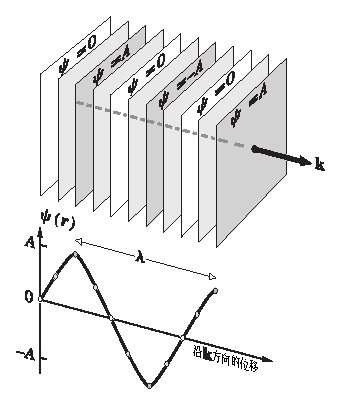
\includegraphics[width=0.5\linewidth]{Pictures/chap08/WavefrontsHarmonicPlaneWave.eps}
    \caption{平面简谐波的波阵面。}
    \label{fig:08ex02.0222}
\end{figure}
如\reffig{08ex02.0222},现在我们构建一组平面,
其上的$\psi(\vec{\mathbf{r}})$于空间中正弦地变化,即
\begin{align}
    \psi(\vec{\mathbf{r}})= & A\sin(\vec{\mathbf{k}}\cdot\vec{\mathbf{r}})\, ,                  \\
    \psi(\vec{\mathbf{r}})= & A\cos(\vec{\mathbf{k}}\cdot\vec{\mathbf{r}})\, ,                  \\
    \psi(\vec{\mathbf{r}})= & A\mathrm{e}^{\mathrm{i}\vec{\mathbf{k}}\cdot\vec{\mathbf{r}}}\, .
\end{align}
显然上面三个式子中,$\psi(\vec{\mathbf{r}})$都在
由$\vec{\mathbf{k}}\cdot\vec{\mathbf{r}}$取常数定义的每个平面上保持恒定。
沿着$\vec{\mathbf{k}}$方向位移$\lambda$后,$\psi$应当在空间中重复。
注意\reffig{08ex02.0222}中只画了无数平面中的若干个,
而平面本身也应无穷延伸,因为扰动充满整个空间。
当平面波在其波阵面上任意处均有相同“强度”时,
我们称其为\keyindex{均匀波}{homogeneous wave}{wave\ 波}。

总之,$\psi$在空间中的周期性可以表示为
\begin{align}
    \psi(\vec{\mathbf{r}})=\psi\left(\vec{\mathbf{r}}+\frac{\lambda}{k}\vec{\mathbf{k}}\right)\, ,
\end{align}
这里$\vec{\mathbf{k}}$也称作\keyindex{传播向量}{propagation vector}{vector\ 向量},
其大小$k$就是传播数\sidenote{类似地,在后文的记号中,如果我们主要想强调一个向量的大小,
    则可能会记作同一字母的标量形式。读者联系上下文即可理解。}。
接着,为了使波运动起来,我们引入时间等变量,最终便得到
\begin{align}\label{eq:08ex02.DirectionCosines}
    \psi(\vec{\mathbf{r}},t)=A\mathrm{e}^{\mathrm{i}(\vec{\mathbf{k}}\cdot\vec{\mathbf{r}}\mp\omega t)}\, .
\end{align}
若$\alpha,\beta$和$\gamma$是$\vec{\mathbf{k}}$在直角坐标系下的方向余弦,则上式还可以写作
\begin{align}
    \psi(x,y,z,t)=A\mathrm{e}^{\mathrm{i}(k(\alpha x+\beta y+\gamma z)\mp\omega t)}
    =A\mathrm{e}^{\mathrm{i}k(\alpha x+\beta y+\gamma z\mp vt)}\, ,
\end{align}
注意
\begin{align}
    \alpha^2+\beta^2+\gamma^2=1\, .
\end{align}

\begin{example}
    试写出平面波$E$的标量表达式:它的振幅为$E_0$,角频率为$\omega$,波长为$\lambda$,
    其传播方向上的单位向量(注意不要混淆为单位基向量$\hat{\text{\sffamily\bfseries k}}$)为
    \begin{align}
        \hat{\mathbf{k}}=\frac{1}{\sqrt{20}}(4\hat{\text{\sffamily\bfseries i}}+2\hat{\text{\sffamily\bfseries j}})\, .
    \end{align}
    我们将该平面波的形式确定为
    \begin{align}
        E(x,y,z,t)=E_0\mathrm{e}^{\mathrm{i}(\vec{\mathbf{k}}\cdot\vec{\mathbf{r}}-\omega t)}\, .
    \end{align}
    这里传播向量$\vec{\mathbf{k}}$满足
    \begin{align}
        \vec{\mathbf{k}}=\frac{\vec{\mathbf{k}}}{|\vec{\mathbf{k}}|}\cdot|\vec{\mathbf{k}}|
        =\hat{\mathbf{k}}\cdot\frac{2\pi}{\lambda}
        =\frac{1}{\sqrt{20}}(4\hat{\text{\sffamily\bfseries i}}+2\hat{\text{\sffamily\bfseries j}})\cdot\frac{2\pi}{\lambda}
        =\frac{\pi}{\sqrt{5}\lambda}(4\hat{\text{\sffamily\bfseries i}}+2\hat{\text{\sffamily\bfseries j}})\, .
    \end{align}
    于是得到$E$的表达式为
    \begin{align}
        E=E_0\mathrm{e}^{\mathrm{i}\left(\displaystyle\frac{\pi}{\sqrt{5}\lambda}(4x+2y)-\omega t\right)}\, .
    \end{align}
\end{example}

\subsubsection*{三维波动微分方程}
像前文推导一维波动微分方程那样,我们可以
类似地用\refeq{08ex02.DirectionCosines}推导出
\begin{definition}[\keyindex{三维波动微分方程}{three-dimensional differential wave equation}{equation\ 方程}]
    \begin{align}\label{eq:08ex02.3d-differential-wave}
        \frac{\partial^2 \psi}{\partial x^2}+\frac{\partial^2 \psi}{\partial y^2}
        +\frac{\partial^2 \psi}{\partial z^2}=\frac{1}{v^2}\frac{\partial^2 \psi}{\partial t^2}\, .
    \end{align}
\end{definition}
注意上式中$x,y$和$z$是对称出现的。引入\keyindex{拉普拉斯算符}{Laplacian operator}{}
\begin{align}
    \nabla^2\equiv\frac{\partial^2}{\partial x^2}
    +\frac{\partial^2}{\partial y^2}+\frac{\partial^2}{\partial z^2}\, ,
\end{align}
则\refeq{08ex02.3d-differential-wave}简化为
\begin{align}\label{eq:08ex02-WaveEquation}
    \nabla^2\psi=\frac{1}{v^2}\frac{\partial^2 \psi}{\partial t^2}\, .
\end{align}
可以证明
\begin{align}
    \psi(\vec{\mathbf{r}},t)=C_1f\left(\frac{1}{k}\vec{\mathbf{k}}\cdot\vec{\mathbf{r}}-vt\right)
    +C_2g\left(\frac{1}{k}\vec{\mathbf{k}}\cdot\vec{\mathbf{r}}+vt\right)
\end{align}
均是上述波动微分方程的平面波解,其中$f$和$g$是二阶可微的任意函数
(不一定为简谐函数),$C_1$和$C_2$是常数。

\subsection{电磁理论}\label{sub:电磁理论}
物理学自19世纪初期以来的发展已经证明了光的是一种电磁波。
在\keyindex{经典电动力学}{classical electrodynamics}{}
的图像中,电磁波是连续传递能量的。但更现代的\keyindex{量子电动力学}{quantum electrodynamics}{}
则用一种质量为零的基本“粒子”来描述电磁相互作用和能量传递,这种粒子称作\keyindex{光子}{photon}{}。
事实证明,光以波的形式在空间中传播,但在发射和吸收时又显出粒子性,即\keyindex{波粒二象性}{wave-particle duality}{}。
电磁辐射的生灭过程是量子化的,但它穿过透镜、小孔等的运动又受波动特性支配。
平均而言,我们可以把大量光子流的平均作用看作是经典电磁波,
这对于\keyindex{物理光学}{physical optics}{optics\ 光学}
而言已经足够处理许多问题了。但请记住电磁波的表观连续性只是宏观层面的假象——事情并不简单,
存在一些情况会使这种描述方法失效。

\subsubsection*{向量场及其积分}
在介绍后续内容前,我们回忆一些关于向量场及其积分的知识。

\keyindex{向量场}{vector field}{},也称\keyindex{矢量场}{}{},
是给其定义域内的每个点都赋有一个向量的函数(如\reffig{08ex02.VelocityVectors})。
直角坐标系下,一个三维空间上的向量场通常形如
\begin{align}
    \vec{\mathbf{F}}(x,y,z)=
    M(x,y,z)\hat{\text{\sffamily\bfseries i}}+
    N(x,y,z)\hat{\text{\sffamily\bfseries j}}+
    P(x,y,z)\hat{\text{\sffamily\bfseries k}}\, ,
\end{align}
其中$M$、$N$和$P$为分量函数;当所有分量函数都连续、可微时,
我们对应称向量场连续、可微。电场和磁场都是向量场。
\begin{figure}[htbp]
    \centering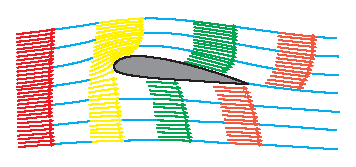
\includegraphics[width=0.4\linewidth]{chap08/VelocityVectors.eps}
    \caption{向量场示例:机翼周围气流的速度场。}
    \label{fig:08ex02.VelocityVectors}
\end{figure}

可微标量函数的梯度给出了该函数在给定点处函数值增长最快的方向,
即每个点都有一个向量与之对应,于是我们定义
\begin{definition}
    可微标量函数$f(x,y,z)$的\keyindex{梯度场}{gradient field}{}
    即为梯度向量构成的场:
    \begin{align}
        \vec{\nabla} f=\text{grad}\ f =\frac{\partial f}{\partial x}\hat{\text{\sffamily\bfseries i}}
        +\frac{\partial f}{\partial y}\hat{\text{\sffamily\bfseries j}}
        +\frac{\partial f}{\partial z}\hat{\text{\sffamily\bfseries k}}\, ,
    \end{align}
    其中$\vec{\nabla}$表示向量微分算符,读作“del”,直角坐标系下为
    \begin{align}
        \vec{\nabla}=\hat{\text{\sffamily\bfseries i}}\frac{\partial }{\partial x}
        +\hat{\text{\sffamily\bfseries j}}\frac{\partial }{\partial y}
        +\hat{\text{\sffamily\bfseries k}}\frac{\partial }{\partial z}\, .
    \end{align}
\end{definition}
$\vec{\nabla}$算符能让我们后续的表示更加方便。

\begin{definition}
    向量场$\vec{\mathbf{F}}(x,y,z)=M(x,y,z)\hat{\text{\sffamily\bfseries i}}+N(x,y,z)\hat{\text{\sffamily\bfseries j}}+P(x,y,z)\hat{\text{\sffamily\bfseries k}}$
    的\keyindex{散度}{divergence}{}
    是标量函数
    \begin{align}
        \text{div}\ \vec{\mathbf{F}}=\vec{\nabla}\cdot\vec{\mathbf{F}}
        =\frac{\partial M}{\partial x}+\frac{\partial N}{\partial y}+\frac{\partial P}{\partial z}\, ,
    \end{align}
\end{definition}
形式上看,散度像是$\vec{\nabla}$算符与向量场点乘得到的。

\begin{definition}
    向量场$\vec{\mathbf{F}}(x,y,z)=M(x,y,z)\hat{\text{\sffamily\bfseries i}}+N(x,y,z)\hat{\text{\sffamily\bfseries j}}+P(x,y,z)\hat{\text{\sffamily\bfseries k}}$
    的\keyindex{旋度}{curl}{}
    向量为
    \begin{align}
        \text{curl}\ \vec{\mathbf{F}}
         & =\vec{\nabla}\times\vec{\mathbf{F}}\nonumber                                                                          \\
         & =\left|
        \begin{array}{ccc}
            \hat{\text{\sffamily\bfseries i}}         & \hat{\text{\sffamily\bfseries j}}         & \hat{\text{\sffamily\bfseries k}}         \\
            \displaystyle\frac{\partial }{\partial x} & \displaystyle\frac{\partial }{\partial y} & \displaystyle\frac{\partial }{\partial z} \\
            M                                         & N                                         & P
        \end{array}
        \right|                                                                                                        \nonumber \\
         & =\left(\frac{\partial P}{\partial y}-\frac{\partial N}{\partial z}\right)\hat{\text{\sffamily\bfseries i}}+
        \left(\frac{\partial M}{\partial z}-\frac{\partial P}{\partial x}\right)\hat{\text{\sffamily\bfseries j}}+
        \left(\frac{\partial N}{\partial x}-\frac{\partial M}{\partial y}\right)\hat{\text{\sffamily\bfseries k}}\, .
    \end{align}
\end{definition}
形式上看,旋度像是$\vec{\nabla}$算符与向量场叉乘得到的。

借助以上定义与符号,我们接着介绍以下数学背景知识。
\begin{definition}
    设向量场$\vec{\mathbf{F}}$定义在开区域$D$上,且对于$D$内的任意两点$A$和$B$,
    曲线积分$\displaystyle\int\limits_C\vec{\mathbf{F}}\cdot\mathrm{d}\vec{\mathbf{\ell}}$
    对所有从$A$到$B$的路径$C$都取值相等,则我们称该积分在$D$上是\keyindex{路径无关的}{path independent}{},
    称$\vec{\mathbf{F}}$在$D$上是\keyindex{保守的}{conservative}{}。
\end{definition}
\begin{definition}
    若定义在区域$D$上的向量场$\vec{\mathbf{F}}$和某个$D$上的标量函数$f$之间满足
    $\vec{\mathbf{F}}=\vec{\nabla} f$,则$f$称作$\vec{\mathbf{F}}$的\keyindex{势函数}{potential function}{}。
\end{definition}

在接下来的相关结论中,我们都约定所讨论的向量场$\vec{\mathbf{F}}$的各分量均有一阶连续偏导数;
曲线是\keyindex{分段光滑}{piecewise smooth}{}
的,它可以计算长度和切向量(除至多有限个点外);
区域$D$是\keyindex{连通的}{connected}{},
个别结论则额外要求它是\keyindex{单连通的}{simply connected}{}。
注意连通和单连通不能相互推出。
\begin{theorem}
    \label{theorem:08ex02-FundamentalTheoremOfLineIntegrals}
    设$C$是空间中从点$A$连接到点$B$的光滑曲线,
    $f$是在包含$C$的区域$D$上定义的可微函数,
    且$f$有连续的梯度场$\vec{\mathbf{F}}=\vec{\nabla} f$,则
    \begin{align}
        \int\limits_C\vec{\mathbf{F}}\cdot\mathrm{d}\vec{\mathbf{\ell}}=f(B)-f(A)\, .
    \end{align}
\end{theorem}
\begin{theorem}
    \label{theorem:08ex02-ConservativeFieldsAreGradientFields}
    设向量场$\vec{\mathbf{F}}$的各分量在整个开连通区域$D$上都连续,
    则当且仅当$\vec{\mathbf{F}}$是某个可微函数$f$的梯度场$\vec{\nabla} f$时,
    $\vec{\mathbf{F}}$是保守的。
\end{theorem}
\begin{theorem}
    \label{theorem:08ex02-LoopPropertyConservativeFields}
    向量场$\vec{\mathbf{F}}$在$D$上是保守的等价于环路积分
    $\displaystyle\oint\limits_C\vec{\mathbf{F}}\cdot\mathrm{d}\vec{\mathbf{\ell}}=0$
    对$D$内的任意闭合曲线$C$恒成立。
\end{theorem}
\begin{theorem}
    \label{theorem:08ex02-ComponentTestForConservativeFields}
    设定义在简单连通开区域上的向量场
    $\vec{\mathbf{F}}(x,y,z)
        =M(x,y,z)\hat{\text{\sffamily\bfseries i}}$\\
    $+N(x,y,z)\hat{\text{\sffamily\bfseries j}}
        +P(x,y,z)\hat{\text{\sffamily\bfseries k}}$
    的各分量均有一阶连续偏导数,则当且仅当以下条件均成立时,$\vec{\mathbf{F}}$是保守的:
    \begin{align}
        \frac{\partial P}{\partial y}=\frac{\partial N}{\partial z}\, ,\quad
        \frac{\partial M}{\partial z}=\frac{\partial P}{\partial x}\, ,\quad
        \frac{\partial N}{\partial x}=\frac{\partial M}{\partial y}\, .
    \end{align}
\end{theorem}
\begin{theorem}[\keyindex{散度定理}{divergence theorem}{}]
    设向量场$\vec{\mathbf{F}}$的各分量均有连续一阶偏导数,
    $S$为有向分片光滑封闭曲面;则$\vec{\mathbf{F}}$沿着$S$曲面上
    朝外的单位法向量场的方向通过曲面的通量等于
    散度$\vec{\nabla}\cdot\vec{\mathbf{F}}$在曲面包围的实区域$D$内的三重积分:
    \begin{align}
        \oiint\limits_S\vec{\mathbf{F}}\cdot\mathrm{d}\vec{\mathbf{S}}
        =\iiint\limits_D\vec{\nabla}\cdot\vec{\mathbf{F}}\mathrm{d}V\, .
    \end{align}
\end{theorem}
\begin{theorem}[\keyindex{斯托克斯定理}{Stokes' theorem}{}]
    设$S$为有向分片光滑曲面,且有分段光滑边界曲线$C$,向量场$\vec{\mathbf{F}}$的各分量
    在一包含$S$的开区域内有连续一阶偏导数;则$\vec{\mathbf{F}}$沿着
    关于曲面单位法向量逆时针的方向绕$C$的环路积分
    等于旋度向量场$\vec{\nabla}\times\vec{\mathbf{F}}$在$S$上的积分:
    \begin{align}
        \oint\limits_C\vec{\mathbf{F}}\cdot\mathrm{d}\vec{\mathbf{\ell}}
        =\iint\limits_A(\vec{\nabla}\times\vec{\mathbf{F}})\cdot\mathrm{d}\vec{\mathbf{S}}\, .
    \end{align}
\end{theorem}
\begin{corollary}
    梯度场的散度恒为零,即
    \begin{align}
        \text{curl}\ \text{grad}\ f=\vec{\nabla}\times\vec{\nabla}f=\vec{0}\, .
    \end{align}
\end{corollary}
\begin{corollary}
    若向量场$\vec{\mathbf{F}}$有连续二阶偏导数,则旋度场的散度恒为零,即
    \begin{align}
        \text{div}\ (\text{curl}\ \vec{\mathbf{F}})=\vec{\nabla}\cdot(\vec{\nabla}\times\vec{\mathbf{F}})=0\, .
    \end{align}
\end{corollary}
\begin{theorem}
    设向量场$\vec{\mathbf{F}}$在简单连通开区域$D$内的任意一点均有
    $\vec{\nabla}\times\vec{\mathbf{F}}=\vec{0}$,
    则它在$D$内的任意分段光滑闭合曲线$C$上的曲线积分恒为0,即
    \begin{align}
        \oint\limits_C\vec{\mathbf{F}}\cdot\mathrm{d}\vec{\mathbf{\ell}}=0\, .
    \end{align}
\end{theorem}

\subsubsection*{电磁理论基本定律}
\keyindex{电荷}{electric charge}{}
是构成物质的基本粒子的一种物理属性,有正负之分,单位为\keyindex{库仑}{coulomb}{}
(库,C)\begin{marginfigure}
    \includegraphics[width=\linewidth]{chap08/CharlesDeCoulomb.jpg}
\end{marginfigure}\sidenote{法国物理学家夏尔·奥古斯丁·德·库仑
    (Charles-Augustin de Coulomb, 1736-1806)。}。
一个\keyindex{质子}{proton}{}
所带的正电荷,或一个\keyindex{电子}{electron}{}
所带的负电荷为\keyindex{基本电荷}{elementary charge}{electric charge\ 电荷},
其值定义为
$e=1.602176634\times10^{-19}\text{C}$.
即便在真空中,电荷也会对彼此施加作用力。
\begin{theorem}[\keyindex{库仑定律}{Coulomb's law}{}]
    真空中两个静止点电荷之间的相互作用力称作\keyindex{静电力}{electrostatic force}{}
    或\keyindex{库仑力}{Coulomb force}{},
    其大小$F$与它们电荷量$q_1$、$q_2$的乘积成正比,
    与它们距离$r$的平方成反比,作用力的方向在它们的连线上;
    同性电荷相斥,异性电荷相吸。该定律的标量形式为
    \begin{align}
        \label{eq:08ex02-CoulombLaw}
        F=\frac{q_1q_2}{4\pi\epsilon_0r^2}\,
    \end{align}
    其中$\epsilon_0$为\keyindex{真空电容率}{vacuum electric permittivity}{permittivity\ 电容率},
    \begin{align}
        \epsilon_0\approx8.85418782\times10^{-12}\text{C}^2/(\text{N}\cdot\text{m}^2)\, ,
    \end{align}
    把系数$k_e$称作\keyindex{静电力常量}{electrostatic force constant}{}
    或\keyindex{库仑常量}{Coulomb's constant}{}:
    \begin{align}
        k_e=\displaystyle\frac{1}{4\pi\epsilon_0}\approx8.9875518\times10^9\text{N}\cdot\text{m}^2/\text{C}^2\, .
    \end{align}
\end{theorem}

我们想象每个电荷都被称作电场的东西包围着,并假设每个电荷与它所沉浸的电场直接相互作用。
\begin{definition}[\keyindex{电场}{electric field}{}]
    若一个点电荷$q$受到电场的力为$\vec{\mathbf{F}}_E$,
    则它所在位置上的电场$\vec{\mathbf{E}}$由
    \begin{align}
        \vec{\mathbf{F}}_E=q\cdot\vec{\mathbf{E}}
    \end{align}
    定义,$\vec{\mathbf{E}}$的大小称作\keyindex{电场强度}{electric field strength}{},
    单位为伏特/米(V/m)或牛顿/库仑(N/C)。
\end{definition}

实验表明两个实际带电体的相互作用力与其自身大小、形状以及电荷分布均有关系。
当带电体之间的距离远大于其自身大小,以致以上因素对它们之间的作用力的影响可以忽略时,
这样的带电体就可以看作是一个点,即\keyindex{点电荷}{point charge}{electric charge\ 电荷}。
电场是在与电荷相互作用中表现其性质的,所以需要将电荷放入电场来研究它。
这个放入的电荷应是电荷量和体积都很小的点电荷,以避免影响原来的电场,便于研究电场各点的性质。
这样的电荷称作\keyindex{检验电荷}{test charge}{electric charge\ 电荷}。
而激发电场的带电体所带的电荷称为\keyindex{源电荷}{source charge}{electric charge\ 电荷}。

除了数学公式,也可以借助图示的方法描述电场。如\reffig{08ex02-electricFieldLine}所示,\keyindex{电场线}{electric field line}{}
是画在电场中有方向的曲线,曲线上每点的切线方向表示该点的电场方向。
因为每点的电场只有一个方向,所以电场线不会相交;线的疏密则反映电场的强弱。
根据电场的定义,它显然满足叠加原理,具有一定分布的电荷各自建立的电场的向量和就是总电场。
\begin{figure}[htbp]
    \centering
    \subfloat[电场线(蓝色)上每点的切线方向表示该点的电场方向。]{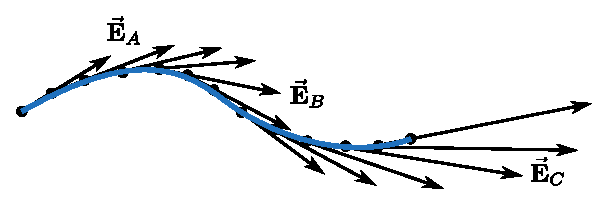
\includegraphics[width=0.65\linewidth]{chap08/FieldLineConstruction.eps}}\\
    \subfloat[正点电荷电场线。]{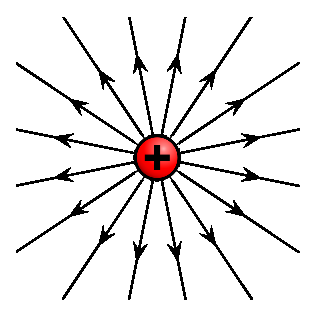
\includegraphics[width=0.27\linewidth]{chap08/electricFieldLinePlusThumb.eps}}\qquad%
    \subfloat[负点电荷电场线。]{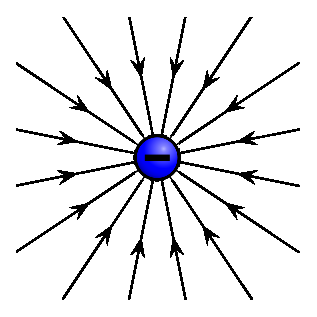
\includegraphics[width=0.27\linewidth]{chap08/electricFieldLineMinusThumb.eps}}\\%
    \subfloat[两个等量同种点电荷和等量异种点电荷之间的电场线。]{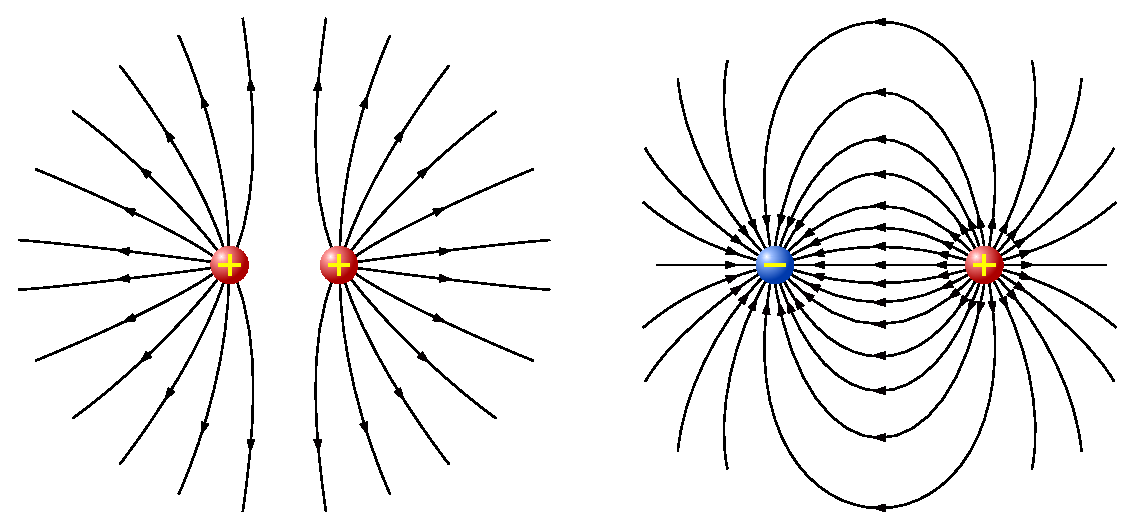
\includegraphics[width=\linewidth]{chap08/electricFieldLine.eps}}\quad%
    \caption{电场线的构建。}
    \label{fig:08ex02-electricFieldLine}
\end{figure}

电场中的电荷具有势能,称作\keyindex{电势能}{electric potential energy}{}。
电势能的数值没有绝对意义,只有相对意义,即需要设定一个电势能为零的参考点,一般取无穷远处的电势能为零。
这样,一个电荷系统的电势能就是其所有电荷被外部作用力从无穷远处移动到现有位置分布且无任何变速过程时所做的总功。
用$W_{AB}$表示检验电荷$q$在电场$\vec{\mathbf{E}}$中沿着路径$C$从点$A$运动到点$B$过程中静电力所做的功,
$E_{pA}$和$E_{pB}$分别表示电荷在点$A$和点$B$处的电势能,则有
\begin{align}
    W_{AB}=\int\limits_{C}q\vec{\mathbf{E}}\cdot\mathrm{d}\vec{\mathbf{\ell}}=E_{pA}-E_{pB}\, .
\end{align}
后文我们将看到,这个功$W_{AB}$与路径$C$无关;而电势能与电荷量之比保持一定,
该比例由电场的性质决定,与检验电荷无关。由此我们定义
\begin{definition}[\keyindex{电势}{electric potential}{}]
    电荷在电场中某点具有的电势$\varphi$等于它在此处的电势能$E_p$与其电荷量$q$的比值:
    \begin{align}
        \label{eq:08ex02-electricPotential}
        \varphi=\frac{E_p}{q}\, .
    \end{align}
\end{definition}
两点之间电势的差值称为\keyindex{电势差}{electrical potential difference}{}
或\keyindex{电压}{voltage}{}。
电势、电势差的单位均为\keyindex{伏特}{volt}{}
(伏,V)\begin{marginfigure}
    \includegraphics[width=\linewidth]{chap08/AlessandroVolta.jpg}
\end{marginfigure}\sidenote{意大利物理学家
    亚历山德罗·朱塞佩·安东尼奥·阿纳斯塔西奥·伏特
    (Alessandro Giuseppe Antonio Anastasio Volta, 1745-1827)。}。
分别记点$A$和点$B$处的电势为$\varphi_{A}$和$\varphi_{B}$,则它们之间的电势差可表示为
\begin{align}
    \label{eq:08ex02-voltage}
    U_{AB} & =\varphi_{A}-\varphi_{B}\, , \\
    U_{BA} & =\varphi_{B}-\varphi_{A}\, .
\end{align}
因此检验电荷$q$从点$A$运动到点$B$静电力所做的功也即
\begin{align}
    W_{AB}=qU_{AB}\, .
\end{align}

根据以上定义,我们能推导出:
\begin{theorem}
    当电场$\vec{\mathbf{E}}$是\keyindex{静电场}{electrostatic field}{}
    时,它是保守场,且是电势$\varphi$的负梯度场
    \begin{align}\label{eq:08ex02-conservativePotential}
        \vec{\mathbf{E}}=-\vec{\nabla}\varphi\, .
    \end{align}
\end{theorem}
\begin{prove}
    当电场$\vec{\mathbf{E}}$是静电场时,所有电场均由电荷建立。
    因为电场满足叠加原理,所以我们不失一般性地只考虑单个点电荷$q$,
    并将其位置设为坐标原点。根据库仑定律\refeq{08ex02-CoulombLaw},
    该电荷在非原点位置$\vec{\mathbf{r}}=x\hat{\text{\sffamily\bfseries i}}+y\hat{\text{\sffamily\bfseries j}}+z\hat{\text{\sffamily\bfseries k}}$处的电场为
    \begin{align}\label{eq:08ex02-DistrubitionElectrostaticField}
        \vec{\mathbf{E}}=\frac{q}{4\pi\epsilon_0|\vec{\mathbf{r}}|^3}\vec{\mathbf{r}}
        =\frac{q}{4\pi\epsilon_0(x^2+y^2+z^2)^{\frac{3}{2}}}(x\hat{\text{\sffamily\bfseries i}}+y\hat{\text{\sffamily\bfseries j}}+z\hat{\text{\sffamily\bfseries k}})\, .
    \end{align}
    可以验证上式满足定理\ref{theorem:08ex02-ComponentTestForConservativeFields},
    所以$\vec{\mathbf{E}}$是保守场,它有一个势函数。
    另一方面,根据前文电势能和电势的内容,有
    \begin{align}
        \int\limits_{C}\vec{\mathbf{E}}\cdot\mathrm{d}\vec{\mathbf{\ell}}
        =\frac{1}{q}\int\limits_{C}q\vec{\mathbf{E}}\cdot\mathrm{d}\vec{\mathbf{\ell}}
        =\frac{1}{q}W_{AB}=\frac{1}{q}(E_{pA}-E_{pB})
        =\varphi_{A}-\varphi_{B}\, .
    \end{align}
    由$A$、$B$和$C$的任意性,对照定理\ref{theorem:08ex02-FundamentalTheoremOfLineIntegrals},
    可知电势取负即$-\varphi$就是电场$\vec{\mathbf{E}}$的势函数。例如,在单个点电荷的电场中,电势为
    \begin{align}\label{eq:08ex02-DistrubitionElectricPotential}
        \varphi(\vec{\mathbf{r}})=\frac{q}{4\pi\epsilon_0|\vec{\mathbf{r}}|}\, .
    \end{align}
\end{prove}

利用\refeq{08ex02-DistrubitionElectricPotential}还能得到:
若是有多个电荷$q_i$各自分布在位置$\vec{\mathbf{r}}_i$,
则从无穷远处将电荷搬运到形成对应分布需要做的功,也即相应电场分布的电势能为
\begin{align}
    W=\sum\limits_{j>1}q_j\left(\sum\limits_{i=1}^{j-1}\frac{q_i}{4\pi\epsilon_0|\vec{\mathbf{r}}_i-\vec{\mathbf{r}}_j|}\right)
    =\frac{1}{2}\sum\limits_{i\neq j}\frac{q_iq_j}{4\pi\epsilon_0|\vec{\mathbf{r}}_i-\vec{\mathbf{r}}_j|}
    =\frac{1}{2}\sum\limits_{i}q_i\varphi_i\, .
\end{align}
其中$\varphi_i$是电荷$q_i$相对于其他所有电荷的电势。上式对于连续电荷分布也适用:
\begin{align}\label{eq:08ex02-PotentialEnergy}
    W=\frac{1}{2}\int\varphi\mathrm{d}q\, .
\end{align}

电势也可以像电场线那样用图示表示。

\begin{definition}
    电场中电势相同的各点构成的面称作\keyindex{等势面}{equipotential surface}{}。
\end{definition}
\begin{corollary}
    电场线与等势面垂直,并且由电势高的等势面指向电势低的等势面。
\end{corollary}

此外,一个运动的电荷还会受到另一种力$\vec{\mathbf{F}}_M$,
称作\keyindex{洛伦兹力}{Lorentz force}{},
它与运动电荷的速度$\vec{\mathbf{v}}$成正比。
为此我们定义另一个场$\vec{\mathbf{B}}$:
\begin{definition}[\keyindex{磁场}{magnetic field}{}]
    它使得
    \begin{align}
        \vec{\mathbf{F}}_M=q\cdot\vec{\mathbf{v}}\times\vec{\mathbf{B}}\, .
    \end{align}
    $\vec{\mathbf{B}}$的大小称作\keyindex{磁感应}{magnetic induction}{}
    强度,单位为\keyindex{特斯拉}{tesla}{}
    (特,T)。
\end{definition}
磁感应强度单位得名于物理学家特斯拉\begin{marginfigure}
    \includegraphics[width=\linewidth]{chap08/TeslaCirca1890.jpg}
\end{marginfigure}\sidenote{塞尔维亚裔美国物理学家
    尼古拉·特斯拉 (Nikola Tesla, 1856-1943)。}。

若电荷在既有电场又有磁场的空间区域内运动,
则会同时受到$\vec{\mathbf{F}}_E$和$\vec{\mathbf{F}}_M$两个力,
合力为$\vec{\mathbf{F}}=q\cdot\vec{\mathbf{E}}+q\cdot\vec{\mathbf{v}}\times\vec{\mathbf{B}}$.
后文我们将看到,随时间变化的磁场会产生电场,随时间变化的电场会产生磁场,
两者的互相依赖性是描述光的关键。

\subsubsection*{法拉第感应定律}
1822年,法拉第\begin{marginfigure}
    \includegraphics[width=\linewidth]{chap08/MichaelFaraday.jpg}
\end{marginfigure}\sidenote{英国物理学家迈克尔·法拉第
    (Michael Faraday, 1791-1867)。}在日记中写下“把磁转换为电”的设想。
1831年,他在线圈实验中发现了\keyindex{电磁感应}{electromagnetic induction}{}
现象,而“变化”是其最实质性的因素。

\begin{figure}[htbp]
    \centering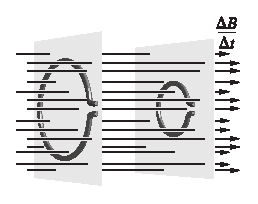
\includegraphics[width=0.4\linewidth]{Pictures/chap08/largerLoopGreaterEmf.eps}
    \caption{更大的环路通过更大的时变磁通量而产生更大的emf。}
    \label{fig:08ex02.0302}
\end{figure}
\begin{figure}[htbp]
    \centering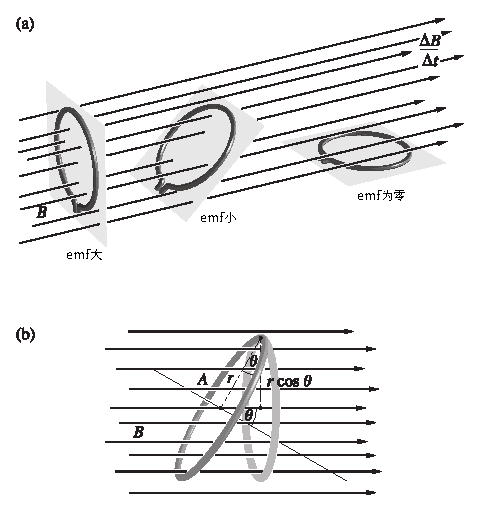
\includegraphics[width=0.75\linewidth]{Pictures/chap08/emfProportionalPerpendicularArea.eps}
    \caption{(a)感生电动势正比于磁场垂直穿过的面积。(b)垂直于磁场的面积随$\cos\theta$变化。}
    \label{fig:08ex02.0303}
\end{figure}

将一根磁铁插进线圈时,
线圈两端会有电压,称作\keyindex{感生电动势}{induced electromotive force}{}
(emf)\sidenote{尽管感生电动势的英文是“force”,
    但它不是力而是电压,故原作者用简称emf避免误解。}。
该电动势的振幅依赖于磁铁运动速度,或者说依赖于穿过线圈的$B$的变化率,而不是$B$本身。
\reffig{08ex02.0302}中,同一变化的$B$场穿过两个不同导线环路,
大的环路两端有更大的感生电动势,即它正比于$B$场垂直穿过的环路面积$A$.
而\reffig{08ex02.0303}中,当环路变倾斜,则垂直于磁场的面积$A_{\perp}$
按$A\cos\theta$变化,其中$\theta$为倾角。当$\theta=90^\circ$时,
没有$B$场穿过环路,感生电动势为零。反之,当磁场恒定时,
感生电动势正比于磁场垂直穿过环路面积的变化率,此外它还正比于$B$.

总之,当$A_{\perp}$恒定时,$\mathrm{emf}\propto A_{\perp}\displaystyle\frac{\Delta B}{\Delta t}$;
当$B$恒定时,$\mathrm{emf}\propto B\displaystyle\frac{\Delta A_{\perp}}{\Delta t}$.
因此,感生电动势依赖于$A_{\perp}$与$B$乘积的变化率。
我们定义穿过导线环路的\keyindex{磁场通量}{flux of the magnetic field}{flux\ 通量}
为
\begin{align}
    \varPhi_M=B_{\perp}A=BA_{\perp}=BA\cos\theta\, ,
\end{align}
其单位为\keyindex{韦伯}{weber}{}
(Wb)\begin{marginfigure}
    \includegraphics[width=\linewidth]{chap08/WilhelmEduardWeber.jpg}
\end{marginfigure}\sidenote{德国物理学家威廉·爱德华·韦伯(Wilhelm Eduard Weber, 1804-1891)。}。

\begin{figure}[htbp]
    \centering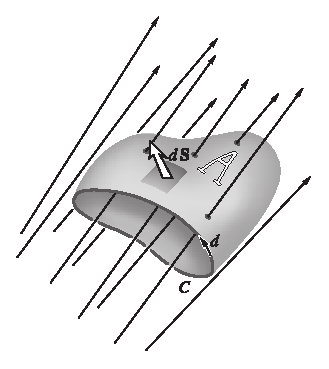
\includegraphics[width=0.5\linewidth]{Pictures/chap08/openAreaBoundedByClosedCurve.eps}
    \caption{$\vec{\mathbf{B}}$场穿过以闭合曲线$C$为边界的非闭合曲面$A$.}
    \label{fig:08ex02.0304}
\end{figure}

如\reffig{08ex02.0304},更一般地,$\vec{\mathbf{B}}$场可能在空间中变化。
穿过导电环路包围的任意非闭合曲面$A$的磁场通量为
\begin{align}
    \varPhi_M=\iint\limits_A\vec{\mathbf{B}}\cdot\mathrm{d}\vec{\mathbf{S}}\, ,
\end{align}
其中$\mathrm{d}\vec{\mathbf{S}}$垂直于曲面朝外。环路上的感生电动势则为
\begin{align}
    \mathrm{emf}=-\frac{\mathrm{d}\varPhi_M}{\mathrm{d}t}\, ,
\end{align}
其中负号说明\begin{marginfigure}
    \includegraphics[width=\linewidth]{chap08/HeinrichFriedrichEmilLenz.jpg}
\end{marginfigure}\sidenote{俄国物理学家
    海因里希·弗里德里希·埃米尔·楞次 (Heinrich Friedrich Emil Lenz, 1804-1865)。}
\begin{theorem}[\keyindex{楞次定律}{Lenz's law}{}]
    感生电动势想要驱动的感生电流,其对应的感生磁场总是想阻碍原先引发它的磁通量的变化。
\end{theorem}

任何一个场中沿着一条闭合曲线的路径积分叫做
该场的\keyindex{环量}{circulation}{}。
电动势也是一种电势差,即单位电荷的电势能之差,
也对应着对单位电荷做的功,或者说对应着电场乘以距离。
电动势只随电场出现:
\begin{align}
    \mathrm{emf}=\oint\limits_C\vec{\mathbf{E}}\cdot\mathrm{d}\vec{\mathbf{\ell}}\, ,
\end{align}
其中积分沿着对应于环路的闭合曲线$C$进行。
联立以上三式可得
\begin{theorem}[\keyindex{法拉第电磁感应定律}{Faraday's law of electromagnetic induction}{}]
    \begin{align}\label{eq:08ex02-FaradayLaw}
        \oint\limits_C\vec{\mathbf{E}}\cdot\mathrm{d}\vec{\mathbf{\ell}}
        =-\frac{\mathrm{d}}{\mathrm{d}t}\iint\limits_A\vec{\mathbf{B}}\cdot\mathrm{d}\vec{\mathbf{S}}\, .
    \end{align}
\end{theorem}
上式除了积分路径$C$外就别无其他物理环路了。
$C$对于是否选在导体内外或附近也没有任何要求。
该式中的电场仅由时变的磁场产生,没有电荷作为电场的\keyindex{源}{source}{}
或\keyindex{汇}{sink}{},所以电场线均自身闭合形成环。

当我们感兴趣的是没有导线回路的空间中传播的电磁波时,
磁通量的变化是完全由$\vec{\mathbf{B}}$引起的,这时感应定律可重写为
\begin{align}\label{eq:08ex02-ElectromagneticInduction}
    \oint\limits_C\vec{\mathbf{E}}\cdot\mathrm{d}\vec{\mathbf{\ell}}
    =-\iint\limits_A\frac{\partial \vec{\mathbf{B}}}{\partial t}\cdot\mathrm{d}\vec{\mathbf{S}}\, .
\end{align}
上式表明一个随时间变化的磁场伴随有一个电场。

\subsubsection*{高斯定律}
电场的另一基本定律即高斯定律\begin{marginfigure}
    \includegraphics[width=\linewidth]{chap08/CarlFriedrichGauss1840.jpg}
\end{marginfigure}\sidenote{德国数学家卡尔·弗里德里希·高斯 (Carl Friedrich Gauss, 1777-1855)。}
描述了电场通量和电荷之间的关系。
场和通量的概念都是从流体动力学引入的。
想象一个闭合曲面隔离出一团运动的流体,例如管道中充盈流动的水,
显然穿过它两个端面的体积流量大小相等,即单位时间内流进来和流出去的量相同。
此时全部表面上相加的流体净流量为零。
但如果有细针插进其中注入或吸走流体,即存在源或汇,则净流量将不再为零。
这种概念同样适用于电场。如\reffig{08ex02.0307}所示,
考虑任意某电场中想象的封闭曲面$A$,
则穿过$A$的\keyindex{电场通量}{flux of the electric field}{flux\ 通量}
为
\begin{align}
    \varPhi_E=\oiint\limits_A\vec{\mathbf{E}}\cdot\mathrm{d}\vec{\mathbf{S}}\, ,
\end{align}
其中带圈的二重积分号强调积分曲面是封闭的,$\mathrm{d}\vec{\mathbf{S}}$垂直于曲面朝外。
当封闭曲面包围的区域内没有电场的源或汇时,电场通量等于零。
\begin{figure}[htbp]
    \centering
    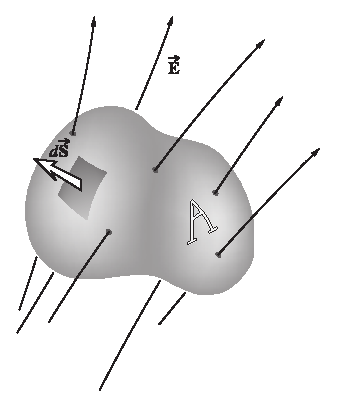
\includegraphics[width=0.5\linewidth]{Pictures/chap08/GausssLawElectric.eps}
    \caption{穿过封闭区域$A$的电场$\vec{\mathbf{E}}$.}
    \label{fig:08ex02.0307}
\end{figure}

当区域内存在源或汇时,考虑任意以正电荷$q$为球心、半径为$r$的球面。
根据库仑定律,该正电荷的电场$\vec{\mathbf{E}}$在球面表面任意处的大小均为
\begin{align}
    E=\frac{1}{4\pi\epsilon_0}\frac{q}{r^2}\, ,
\end{align}
且都沿径向向外垂直于球面表面,即$\vec{\mathbf{E}}=\vec{\mathbf{E}}_\perp$.
于是
\begin{align}
    \varPhi_E=\oiint\limits_A\vec{\mathbf{E}}\cdot\mathrm{d}\vec{\mathbf{S}}
    =\oiint\limits_A E_\perp\mathrm{d}S
    =E\oiint\limits_A\mathrm{d}S=4\pi r^2E=\frac{q}{\epsilon_0}\, .
\end{align}
以上推导也适用于负电荷,推广到区域内的多个电荷时,将上式累加即可:
\begin{align}
    \varPhi_E=\frac{1}{\epsilon_0}\sum q\, .
\end{align}
把电荷分布近似为连续分布,在$A$所包围的体积$V$内,记电荷分布体密度为$\rho$
(在线上分布的线密度或在面上分布的面密度也同理),则最终得到
\begin{theorem}[电场的\keyindex{高斯定律}{Gauss's Law}{}]
    穿过任意封闭曲面的净电场通量正比于它包围的净电荷量。
    \begin{align}\label{eq:08ex02.GausssLawElectric}
        \oiint\limits_A\vec{\mathbf{E}}\cdot\mathrm{d}\vec{\mathbf{S}}
        =\frac{1}{\epsilon_0}\iiint\limits_V\rho\mathrm{d}V\, .
    \end{align}
\end{theorem}

\refeq{08ex02.GausssLawElectric}使用了\keyindex{自由空间}{free space}{}
的真空电容率$\epsilon_0$,若电荷嵌在某种实物介质中,
则须用该介质的\keyindex{电容率}{permittivity}{}
$\epsilon$替代$\epsilon_0$;
然而电容率又是描述平行板电容器的的基础概念,单位制的差异
引发了$\epsilon$的取值问题。为了避免这些麻烦,
我们定义一个与单位制无关的新物理量,即\keyindex{相对电容率}{relative permittivity}{permittivity\ 电容率}
$K_E$,也称\keyindex{相对介电常数}{relative dielectric constant}{}:
\begin{align}\label{eq:08ex02-relativepermittivity}
    K_E=\frac{\epsilon}{\epsilon_0}\, ,
\end{align}
显然真空的$K_E$为1,它是无量纲的。

目前物理界尚未发现与电荷对应的“磁荷”存在,没有发现过孤立的磁极(磁单极)。
磁场$\vec{\mathbf{B}}$的磁力线总是连续和闭合的。因此对于磁场中的任何封闭曲面,
由于其中不存在任何磁单极,所以进入和离开的磁力线数目保持相等(如\reffig{08ex02.0308}),
穿过该曲面的磁通量$\varPhi_M$为零。于是我们得到
\begin{theorem}[磁场的高斯定律]
    磁场中的任何封闭曲面的净磁通量为零。
    \begin{align}\label{eq:08ex02-GausssLawMagnetic}
        \oiint\limits_A\vec{\mathbf{B}}\cdot\mathrm{d}\vec{\mathbf{S}}=0\, .
    \end{align}
\end{theorem}
\begin{figure}[htbp]
    \centering
    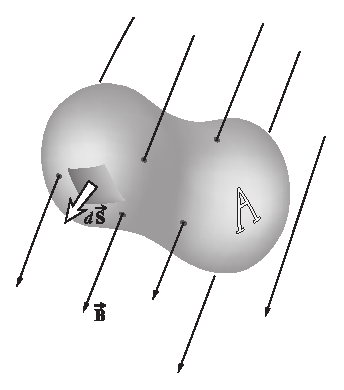
\includegraphics[width=0.5\linewidth]{Pictures/chap08/GausssLawMagnetic.eps}
    \caption{穿过封闭区域$A$的磁场$\vec{\mathbf{B}}$.}
    \label{fig:08ex02.0308}
\end{figure}

\begin{example}
    如\reffig{08ex02-sphereField},若自由空间中一个半径为$R$的实心球体均匀带电,总电荷量为$Q$,求相应的电场分布。
    \begin{figure}[htbp]
        \centering
        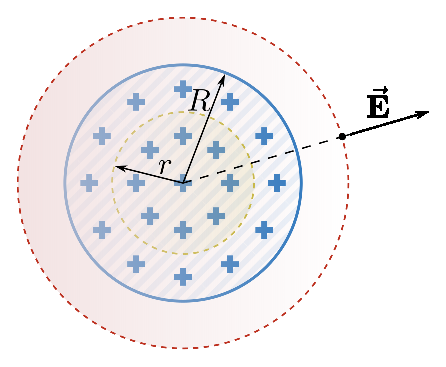
\includegraphics[width=0.4\linewidth]{chap08/sphereElectricField.eps}
        \caption{均匀带电实心球体的电场。}
        \label{fig:08ex02-sphereField}
    \end{figure}

    首先,容易求得该球体的电荷体密度为
    \begin{align}
        \rho=\frac{Q}{\displaystyle\frac{4}{3}\pi R^3}\, .
    \end{align}
    以该球体的球心为原点,记任一位置的位移矢量为$\vec{\mathbf{r}}$,对应电场为$\vec{\mathbf{E}}$.
    显然由本问题的几何对称性,当$Q$为正或负时,$\vec{\mathbf{E}}$的方向与$\vec{\mathbf{r}}$同向或反向。
    把$\vec{\mathbf{E}}$带符号的大小记作$E_r$,作一个与带电球体同心且半径为$r$的封闭球面(图中黄色或红色球),
    则根据高斯定律\refeq{08ex02.GausssLawElectric}有
    \begin{align}
        4\pi r^2E_r
        =\left\{\begin{array}{ll}
            \displaystyle\frac{4}{3\epsilon_0}\pi r^3\rho=\left(\frac{r}{R}\right)^3\frac{Q}{\epsilon_0}, & \text{当}r<R,    \\
            \displaystyle\frac{4}{3\epsilon_0}\pi R^3\rho=\frac{Q}{\epsilon_0},                           & \text{当}r\ge R.
        \end{array}\right.
    \end{align}
    整理得到
    \begin{align}
        E_r=\left\{\begin{array}{ll}
            \displaystyle\frac{Qr}{4\pi\epsilon_0R^3}, & \text{当}r<R,    \\
            \displaystyle\frac{Q}{4\pi\epsilon_0r^2},  & \text{当}r\ge R.
        \end{array}\right.
    \end{align}
    所以电场分布为
    \begin{align}
        \vec{\mathbf{E}}=\left\{\begin{array}{ll}
            \displaystyle\frac{Q}{4\pi\epsilon_0R^3}\vec{\mathbf{r}}, & \text{当}r<R,    \\
            \displaystyle\frac{Q}{4\pi\epsilon_0r^3}\vec{\mathbf{r}}, & \text{当}r\ge R.
        \end{array}\right.
    \end{align}
\end{example}

\begin{example}
    自由空间中,两块无限大的均匀带电平板平行放置,形成理想平行板电容器。
    其中一块平板的电荷面密度为$+\sigma>0$,另一块的为$-\sigma$,
    忽略平板厚度和边缘效应,求空间中的电场分布。
    \begin{figure}[htbp]
        \centering
        \subfloat[单块无限大均匀带电板的电场。]{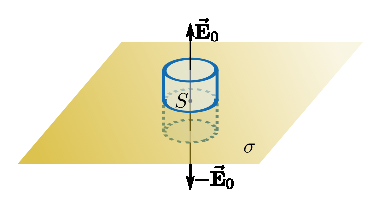
\includegraphics[width=0.45\linewidth]{chap08/SingleSheets.eps}}\quad%
        \subfloat[两块无限大均匀带电板的电场。]{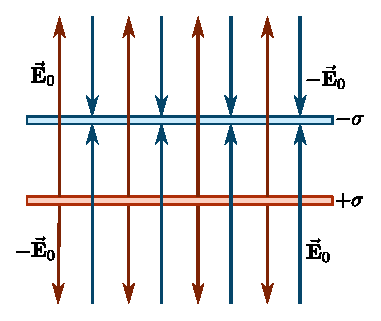
\includegraphics[width=0.45\linewidth]{chap08/ParallelSheets.eps}}%
        \caption{理想平行板电容器的电场。}
        \label{fig:08ex02-ParallelSheets}
    \end{figure}

    如\reffig{08ex02-ParallelSheets}(a),先考虑单块均匀带电平板的电场$\vec{\mathbf{E}}_0$.
    由几何对称性,电场的方向应处处垂直于平板,当平板带正电或负电时,平板两侧电场的方向均远离或接近平板。
    以带正电为例,任取一个极小圆柱体与平板相交,圆柱体底面与平板平行,截面积为$S$,则圆柱体包围的电荷为$\sigma S$.
    根据高斯定律\refeq{08ex02.GausssLawElectric}有
    \begin{align}
        2E_0S=\frac{\sigma S}{\epsilon_0}\, .
    \end{align}
    所以
    \begin{align}
        E_0=\frac{\sigma}{2\epsilon_0}\, .
    \end{align}
    以上结论对带负电的情况也适用。如\reffig{08ex02-ParallelSheets}(b),
    同时考虑两块带相反等量电荷的平板时,将二者的电场叠加即可。易得两板之间的电场同向叠加为
    \begin{align}\label{eq:08ex02-ParallelSheets}
        E=E_0+E_0=\frac{\sigma}{\epsilon_0}\, .
    \end{align}
    其方向从正电板指向负电板,且与之垂直;而两板外侧的电场则反向抵消为
    \begin{align}
        E=E_0+(-E_0)=0\, .
    \end{align}

    对于面积有限的平行板电容器,适当条件下可类比以上情况作近似处理。
    记每块平板面积为$A$,板间介电质材料的电容率为$\epsilon$,
    充电后的电压为$U$,板间距离为$d$,则它的\keyindex{电容}{capacitance}{}
    为
    \begin{align}\label{eq:08ex02-capacitanceParallel}
        C=\frac{\sigma A}{U}=\frac{\sigma A}{Ed}=\frac{\sigma A}{\displaystyle\frac{\sigma}{\epsilon}d}=\frac{\epsilon A}{d}\, .
    \end{align}
    其单位为\keyindex{法拉}{farad}{}
    (法,F)\sidenote{得名于法拉第。}。结合\refeq{08ex02-PotentialEnergy},
    还能得到电容器存储的能量为
    \begin{align}\label{eq:08ex02-ParallelEnergy}
        W=\frac{1}{2}\sigma AU=\frac{1}{2}\frac{\sigma A}{U}U^2
        =\frac{1}{2}\frac{\sigma A}{Ed}U^2
        =\frac{1}{2}\frac{\sigma A}{\displaystyle\frac{\sigma}{\epsilon}d}U^2
        =\frac{1}{2}CU^2\, .
    \end{align}
\end{example}

\subsubsection*{安培环路定律}
如\reffig{08ex02.0309}所示,一根电流为$i$的载流直导线形成了环绕它的磁场$\vec{\mathbf{B}}$,
实验表明磁场大小为
\begin{align}\label{eq:08ex02-BfieldCurrentWire}
    B=\frac{\mu_0i}{2\pi r}\, ,
\end{align}
其中常数$\mu_0$的含义稍后介绍,$r$为半径大小。

在19世纪时,物理学界认为磁荷是存在的,于是我们定义单级磁荷$q_m$,
它在磁场$\vec{\mathbf{B}}$中受到的力等于$q_m\vec{\mathbf{B}}$,
方向在$\vec{\mathbf{B}}$的方向上,就像电场$\vec{\mathbf{E}}$中的
电荷$q_e$所受的力$q_e\vec{\mathbf{E}}$那样。
假设该磁荷指北,并被放到一条以载流直导线为圆心且垂直于导线的闭合圆形轨道上,
围绕着导线运动,我们考察该过程磁场所做的功。
注意到\refeq{08ex02-BfieldCurrentWire},
因为轨道上任意一点到圆心的距离恒定,所以磁场大小相等,
且方向处处与轨道相切,即磁感应强度沿轨道切向的分量大小为$B_{\parallel}=B$.
任取一小段轨道$\Delta\ell$,则该段内磁场做功为$\Delta W=q_mB_{\parallel}\Delta\ell$,将每一小段求和得
\begin{align}
    \sum q_mB_{\parallel}\Delta\ell=q_mB\sum\Delta\ell=q_m\frac{\mu_0i}{2\pi r}\cdot2\pi r=q_m\mu_0i\, .
\end{align}
注意到上式中半径$r$被抵消了,即做的功和具体在哪条圆形轨道上无关;
若磁荷沿着半径方向运动,则因位移垂直于$\vec{\mathbf{B}}$而不做功。
于是我们在磁荷绕圈时将它从一个圆周上搬运到另一个圆周上,做的功必定相同。
也就是说,功与路径完全无关,在围绕电流的任何闭合路径上做的功都相同。
\begin{figure}[htbp]
    \centering
    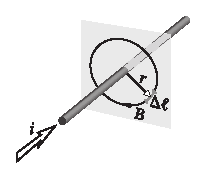
\includegraphics[width=0.3\linewidth]{Pictures/chap08/BfieldCurrent-carryingWire.eps}
    \caption{磁场$\vec{\mathbf{B}}$环绕着载流直导线。}
    \label{fig:08ex02.0309}
\end{figure}

约去磁荷$q_m$,我们得到求和式:
\begin{align}
    \sum B_{\parallel}\Delta\ell=\mu_0i\, .
\end{align}
它对围绕电流的任意闭合路径都成立。
注意这个式子的成立不依赖于假设的单极磁荷,
我们不需要借助磁荷这个假想概念了。
它还可以推广到闭合路径包围的载流导线不止一根的情形——
各个电流的磁场会叠加起来形成总磁场,而上式对总磁场也成立,即
\begin{align}
    \sum B_{\parallel}\Delta\ell=\mu_0\sum i\, ,
\end{align}
令$\Delta\ell\rightarrow0$,则上式化为积分
\begin{align}
    \oint\limits_C\vec{\mathbf{B}}\cdot\mathrm{d}\vec{\mathbf{\ell}}=\mu_0\sum i\, ,
\end{align}
这就是安培定律\begin{marginfigure}
    \includegraphics[width=\linewidth]{chap08/AmpereAndre1825.jpg}
\end{marginfigure}\sidenote{法国物理学家安德烈-马里·安培 (André-Marie Ampère, 1775-1836)。}。
它将$\vec{\mathbf{B}}$沿着闭合曲线$C$切向的线积分
与$C$包围区域内的电流联系起来。当电流不均匀地流过截面时,
安培定律右边可改写成\keyindex{电流密度}{current density}{}
$\vec{\mathbf{J}}$在截面面积上的积分:
\begin{align}
    \oint\limits_C\vec{\mathbf{B}}\cdot\mathrm{d}\vec{\mathbf{\ell}}
    =\mu_0\iint\limits_A\vec{\mathbf{J}}\cdot\mathrm{d}\vec{\mathbf{S}}\, ,
\end{align}
其中非封闭区域$A$以$C$为边界(如\reffig{08ex02.0310}),
常数$\mu_0$称作\keyindex{真空磁导率}{vacuum magnetic permeability}{permeability\ 磁导率}:
\begin{align}
    \mu_0\approx4\pi\times10^{-7}\approx1.256637061\times10^{-6}\text{N}\cdot\text{s}^2/\text{C}^2
\end{align}
若在实物介质中,则换成对应介质的\keyindex{磁导率}{permeability}{} $\mu$.
类似于\refeq{08ex02-relativepermittivity},
我们定义无量纲的\keyindex{相对磁导率}{relative permeability}{permeability\ 磁导率}
为
\begin{align}
    K_M=\frac{\mu}{\mu_0}\, .
\end{align}
\begin{figure}[htbp]
    \centering
    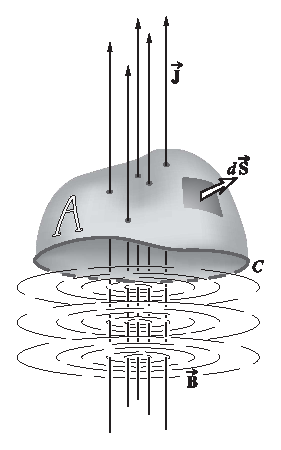
\includegraphics[width=0.4\linewidth]{Pictures/chap08/CurrentDensityThroughArea.eps}
    \caption{通过非封闭区域$A$的电流密度。}
    \label{fig:08ex02.0310}
\end{figure}

安培定律并没有具体规定区域$A$,而只需要它以$C$为边界即可。
在电容器充电的例子中,这会产生新的问题。如\reffig{08ex02.0311}(a),
若选择面$A_1$,则有净电流$i$穿过它,因而存在沿着曲线$C$的磁场;
若选择面$A_2$,则没有净电流流过,沿$C$的磁场必须为零;显然这里出现了矛盾。
\begin{figure}[htbp]
    \centering
    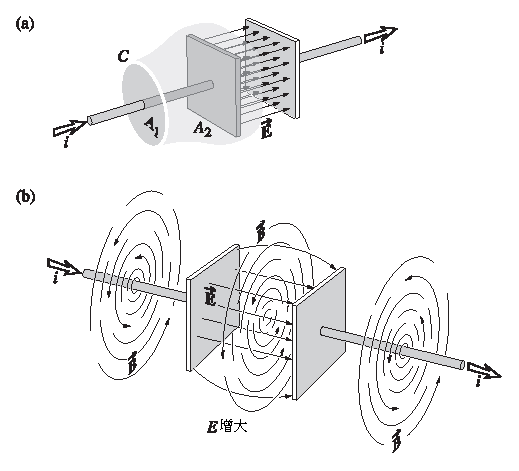
\includegraphics[width=0.8\linewidth]{Pictures/chap08/AmperesLawCapacitor.eps}
    \caption{(a)安培定律不在乎以$C$为边界的区域是$A_1$还是$A_2$,
        但电流只穿过$A_1$没穿过$A_2$,引发了矛盾;
        (b)在电容器极板之间,$\vec{\mathbf{B}}$场伴随着时变的$\vec{\mathbf{E}}$场出现。}
    \label{fig:08ex02.0311}
\end{figure}

并不是只有运动电荷才能产生磁场。如\reffig{08ex02.0311}(b),
当给电容器充电或放电时,虽然没有实际电流流过电容器,
但其极板间也可以测量到磁场,且和引线周围的磁场无法区分。
设每块极板的面积为$A$,电荷量为$Q$,则电场强度为
\begin{align}
    E=\frac{Q}{\epsilon A}\, .
\end{align}
当电荷量变化时,电场也随之变化,上式两边对时间$t$求导并整理后得
\begin{align}
    \epsilon\frac{\partial E}{\partial t}=\frac{i}{A}\, ,
\end{align}
这说明$\displaystyle\epsilon\frac{\partial E}{\partial t}$等效于电流密度。
麦克斯韦\begin{marginfigure}
    \includegraphics[width=\linewidth]{chap08/James-Clerk-Maxwell-1831-1879.jpg}
\end{marginfigure}\sidenote{英国物理学家詹姆斯·克拉克·麦克斯韦(James Clerk Maxwell, 1831-1879)。}
提出该概念,并称作\keyindex{位移电流密度}{displacement current density}{current density\ 电流密度},
定义为
\begin{align}
    \vec{\mathbf{J}}_D=\epsilon\frac{\partial\vec{\mathbf{E}}}{\partial t}\, .
\end{align}
于是我们将以上结论重新表述为
\begin{theorem}[\keyindex{Ampère's Circuital Law}{安培环路定律}{}]
    对于以闭合路径$C$为边界的任意非封闭曲面$A$,有
    \begin{align}\label{eq:08ex02-AmpereLaw}
        \oint\limits_C\vec{\mathbf{B}}\cdot\mathrm{d}\vec{\mathbf{\ell}}
        =\mu\iint\limits_A\left(\vec{\mathbf{J}}
        +\epsilon\frac{\partial\vec{\mathbf{E}}}{\partial t}\right)
        \cdot\mathrm{d}\vec{\mathbf{S}}\, ,
    \end{align}
\end{theorem}
这是麦克斯韦最伟大的贡献之一,表明了即使$\vec{\mathbf{J}}$为零,
一个时变的电场$\vec{\mathbf{E}}$也会伴随一个磁场$\vec{\mathbf{B}}$(\reffig{08ex02.0312})。
\begin{figure}[htbp]
    \centering
    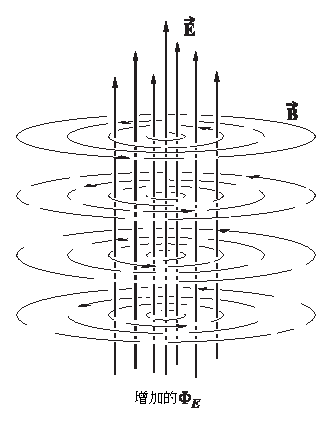
\includegraphics[width=0.5\linewidth]{Pictures/chap08/time-varyingE-field.eps}
    \caption{时变的电场$\vec{\mathbf{E}}$. 磁场$\vec{\mathbf{B}}$围绕
        着$\varPhi_E$变化的每一点形成闭环。向上增加的电场等效于向上的位移电流。
        根据右手定则,感生磁场$\vec{\mathbf{B}}$在从上往下看时逆时针旋转。}
    \label{fig:08ex02.0312}
\end{figure}

\subsubsection*{麦克斯韦方程组}
\refeq{08ex02-ElectromagneticInduction}、\refeq{08ex02.GausssLawElectric}、
\refeq{08ex02-GausssLawMagnetic}与\refeq{08ex02-AmpereLaw}给出的式子
称作积分形式的麦克斯韦方程组,它们是对实验结果的概括。
自由空间中的电场和磁场行为对应于麦克斯韦方程组的最简形式:
当$\epsilon=\epsilon_0$且$\mu=\mu_0$时,
假设没有电流,附近也无电荷,即$\rho$和$\vec{\mathbf{J}}$都为零,则此时有
\begin{align}
    \oint\limits_C\vec{\mathbf{E}}\cdot\mathrm{d}\vec{\mathbf{\ell}}
                                                                   & =-\iint\limits_A\frac{\partial \vec{\mathbf{B}}}{\partial t}\cdot\mathrm{d}\vec{\mathbf{S}}\, , \\
    \oint\limits_C\vec{\mathbf{B}}\cdot\mathrm{d}\vec{\mathbf{\ell}}
                                                                   & =\mu_0\epsilon_0\iint\limits_A\frac{\partial\vec{\mathbf{E}}}{\partial t}
    \cdot\mathrm{d}\vec{\mathbf{S}}\, ,                                                                                                                              \\
    \oiint\limits_A\vec{\mathbf{B}}\cdot\mathrm{d}\vec{\mathbf{S}} & =0\, ,                                                                                          \\
    \oiint\limits_A\vec{\mathbf{E}}\cdot\mathrm{d}\vec{\mathbf{S}} & =0\, .
\end{align}
从中可以看到,除了相乘的标量因子外,电场和磁场在上面的方程中具有明显的对称性。
电场怎样影响磁场,磁场也怎样反过来影响电场。

利用散度定理和斯托克斯定理,麦克斯韦方程组可重新写为微分形式:
\begin{theorem}[真空中的\keyindex{麦克斯韦方程组}{Maxwell's equations}{}]
    \begin{align}
        \label{eq:08ex02-MaxwellFaraday}\text{法拉第电磁感应定律:} &  & \vec{\nabla}\times\vec{\mathbf{E}} & =-\frac{\partial \vec{\mathbf{B}}}{\partial t}\, ,                                             \\
        \label{eq:08ex02-MaxwellAmpere}\text{安培环路定律:}        &  & \vec{\nabla}\times\vec{\mathbf{B}} & =\mu_0\left(\vec{\mathbf{J}}+\epsilon_0\frac{\partial \vec{\mathbf{E}}}{\partial t}\right)\, , \\
        \label{eq:08ex02-MaxwellGaussE}\text{电场的高斯定律:}      &  & \vec{\nabla}\cdot\vec{\mathbf{E}}  & =\frac{\rho}{\epsilon_0}\, ,                                                                   \\
        \label{eq:08ex02-MaxwellGaussB}\text{磁场的高斯定律:}      &  & \vec{\nabla}\cdot\vec{\mathbf{B}}  & =0\, .
    \end{align}
\end{theorem}

特别地,在静电场中,导电物体表面的电势受外部源的约束,
其表面电荷分布及其引发的部分电场难以直接求得。
而电荷分布和电场分布又相互影响,所以求解的结果应保证自洽性。
但要用上述积分定律做到这点有时会比较难算,而改用场的微分形式则更简单——
将\refeq{08ex02-MaxwellGaussE}代入\refeq{08ex02-conservativePotential}得\begin{marginfigure}
    \includegraphics[width=\linewidth]{chap08/SimeonDenisPoisson.jpg}
\end{marginfigure}\sidenote{法国数学家、物理学家西梅翁·德尼·泊松 (Siméon Denis Poisson, 1781-1840)。}
\begin{theorem}[\keyindex{泊松方程}{Poisson's equation}{}]
    静电场的电势$\varphi$满足
    \begin{align}
        \vec{\nabla}\cdot(\vec{\nabla}\varphi)=\nabla^2\varphi=-\frac{\rho}{\epsilon_0}\, .
    \end{align}
\end{theorem}
其中$\nabla^2$是拉普拉斯算符;特别地,在零电荷区域内,泊松方程化为
\begin{marginfigure}
    \includegraphics[width=\linewidth]{chap08/Laplace.jpg}
\end{marginfigure}\sidenote{法国数学家皮埃尔-西蒙·拉普拉斯 (Pierre-Simon, Marquis de Laplace, 1749-1827)。}
\begin{theorem}[\keyindex{拉普拉斯方程}{Laplace's equation}{}]
    \begin{align}
        \nabla^2\varphi=0\, .
    \end{align}
\end{theorem}

有了以上知识,我们就能理解电磁波的传播了。
在该过程中,电场和磁场不可分割地耦合在一起并相互维持,
作为一个整体在空间中传播,不依赖电荷、电流、实物介质或以太。

\subsubsection*{电磁波}
我们已经知道,时变的电场产生磁场,磁场处处垂直于电场变化的方向;
时变的磁场产生电场,电场处处垂直于磁场变化的方向。
考虑一个从静止状态加速运动的电荷,电荷附近的电场发生变化,
该变化以某个有限速度向外传播;因为电荷的运动是加速的,
电场随时间的变化率不是常数,所以感生的磁场也是时变的,
于是又产生一个电场……这个过程继续下去,电场和磁场耦合为一个脉冲,
互相不断变化产生,在空间中传播。

我们可以把电场和磁场看成是单一的物理现象——\keyindex{电磁场}{electromagnetic field}{}
的两个方面,它的源是运动电荷。一旦电磁场中有扰动生成,
就成为不受约束的波,脱离波源独立运动,即\keyindex{电磁波}{electromagnetic wave}{wave\ 波}。
可以证明,自由空间的麦克斯韦方程组可以推导出以下两个表达式:
\begin{align}
    \label{eq:08ex02-WaveElectric}
    \nabla^2\vec{\mathbf{E}} & =\epsilon_0\mu_0\frac{\partial^2\vec{\mathbf{E}}}{\partial t^2}\, , \\
    \nabla^2\vec{\mathbf{B}} & =\epsilon_0\mu_0\frac{\partial^2\vec{\mathbf{B}}}{\partial t^2}\, .
\end{align}
这里它作用于向量场表示分别作用于其每个分量;
偏微分算符同理(故上面两式总共可拆为六个分量方程)。
注意与\refeq{08ex02-WaveEquation}比较,
可发现电磁场服从波动方程,同时还预言了自由空间里所有电磁波的波速为
\begin{align}\label{eq:08ex02-speedOfLight}
    v=\frac{1}{\sqrt{\epsilon_0\mu_0}}\approx3\times10^8\text{m}/\text{s}\, .
\end{align}
这个理论值和斐索\begin{marginfigure}
    \includegraphics[width=\linewidth]{chap08/ArmandHippolyteLouisFizeau.jpg}
\end{marginfigure}\sidenote{法国物理学家阿尔芒·伊波利特·路易·斐索 (Armand Hippolyte Louis Fizeau, 1819-1896)。}
用旋转齿轮法测到的光速值(315300km/s)符合得很好。麦克斯韦由此断定:光就是一种电磁波!
1887年,赫兹首次用实验证明了电磁波的存在。这是物理学上划时代的卓越发现!

现在习惯上用$c$表示真空中的光速,它取自拉丁文“celer”,意思是“快”。
1983年在巴黎召开的第17届国际计量大会\sidenote{the 17th Conférence Générale des Poids et Mesures}
规定了长度单位“米”的新定义,即把真空中的光速精确设定为
\begin{align}
    c=2.99792458\times10^8\text{m}/\text{s}\, .
\end{align}
2019年5月20日起新生效的国际单位制基本单位已要求\refeq{08ex02-speedOfLight}严格成立,
真空电容率$\epsilon_0$和真空磁导率$\mu_0$的测定值由此绑定。
注意\refeq{08ex02-speedOfLight}给出的光速与光源和观察者的运动无关,
这很不平常,但却没人注意,直到1905年爱因斯坦提出\keyindex{狭义相对论}{special relativity}{}。

下面我们利用电磁理论解释实验证实的光的横波特性。
考虑真空中朝正$x$方向传播的平面波这一简单情形,
电场$\vec{\mathbf{E}}=E_x\hat{\text{\sffamily\bfseries i}}+E_y\hat{\text{\sffamily\bfseries j}}+E_z\hat{\text{\sffamily\bfseries k}}$是\refeq{08ex02-WaveElectric}的解,
且因为是平面波,所以在垂直于$x$轴的任意平面上$\vec{\mathbf{E}}$是恒定的。
因此它只是$x$和时间$t$的函数,即$\vec{\mathbf{E}}=\vec{\mathbf{E}}(x,t)$,
于是有$\displaystyle\frac{\partial E_y}{\partial y}=\frac{\partial E_z}{\partial z}=0$恒成立。
代入麦克斯韦方程组的\refeq{08ex02-MaxwellGaussE}(这里$\rho=0$),可得
\begin{align}
    \displaystyle\frac{\partial E_x}{\partial x}=0\, .
\end{align}
若$E_x$是非零值,则意味着电场在传播的$x$方向上有分量,且不随$x$变化。
于是在任一给定时刻,所有$x$上的$E_x$都相等,可这就意味着不存在沿$x$方向传播的行波,矛盾!
故$E_x$只能是零,在其传播方向上没有电场分量,只能是横波。
\begin{figure}[htbp]
    \centering
    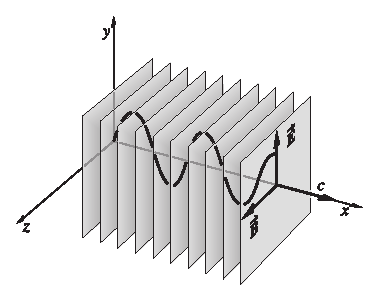
\includegraphics[width=0.5\linewidth]{Pictures/chap08/planeHarmonicElectromagneticWave.eps}
    \caption{真空中传播的平面简谐电磁波。}
    \label{fig:08ex02.0313}
\end{figure}

电场是横波意味着,我们如果要完备描述电磁波,就须规定各个时刻$\vec{\mathbf{E}}$的方向,
这对应了光的\keyindex{偏振}{polarization}{}。不失一般性地,
这里主要讨论平面波或线性偏振波,
此时$\vec{\mathbf{E}}$的震动方向是固定的。
我们不妨取定坐标轴方向使得电场平行于$y$轴(如\reffig{08ex02.0313}),于是
\begin{align}
    \vec{\mathbf{E}}=\hat{\text{\sffamily\bfseries j}}E_y(x,t)\, ,
\end{align}
代入麦克斯韦方程组的\refeq{08ex02-MaxwellFaraday},
注意$E_x=E_z=0$且$E_y$与$x$和$z$无关,得
\begin{align}\label{eq:08ex02-EyBz}
    \frac{\partial E_y}{\partial x}=-\frac{\partial B_z}{\partial t}\, .
\end{align}
而$B_x$和$B_y$是恒定的,这里我们不关心它。
于是依赖于时间$t$的磁场$\vec{\mathbf{B}}$只能有一个$z$方向的分量。
所以,在自由空间里,平面电磁波是横波。除了正入射外,
在真实实物介质中传播的这种波有时不是横波,这种复杂情况
可能是介质是耗散的或含有自由电荷引发的。
这里我们暂时只讨论均匀、各向同性、线性且稳定的介电质(即不导电),
此时平面电磁波是横波。

除了假设扰动是平面波外,我们没有规定其具体形式,
所以结论是具有普遍性的,脉冲和连续波都适用。
因为任意波形都能分解为正弦波,所以我们就限于讨论简谐波,不妨取
\begin{align}\label{eq:08ex02-Eyxt}
    E_y(x,t)=E_{0y}\cos\left(\omega\left(t-\frac{x}{c}\right)+\varepsilon\right)\, ,
\end{align}
其传播速度为$c$,代入\refeq{08ex02-EyBz}得
\begin{align}
    B_z(x,t)=-\int\frac{\partial E_y}{\partial x}\mathrm{d}t
    =\frac{1}{c}E_{0y}\cos\left(\omega\left(t-\frac{x}{c}\right)+\varepsilon\right)\, ,
\end{align}
这里舍去了表示与时间无关的场的积分常数。与\refeq{08ex02-Eyxt}比较可知,在真空中有
\begin{align}\label{eq:08ex02-EycBz}
    E_y=cB_z\, .
\end{align}
因为$E_y$和$B_z$只差一个标量因子,所以具有相同的时间依赖关系,
$\vec{\mathbf{E}}$和$\vec{\mathbf{B}}$在空间中所有位置上同相。
此外,$\vec{\mathbf{E}}=\hat{\text{\sffamily\bfseries j}}E_y(x,t)$和$\vec{\mathbf{B}}=\hat{\text{\sffamily\bfseries k}}B_z(x,t)$互相垂直,
它们的叉乘$\vec{\mathbf{E}}\times\vec{\mathbf{B}}$指向传播方向$\hat{\text{\sffamily\bfseries i}}$
(如\reffig{08ex02.0314})。
\begin{figure}[htbp]
    \centering
    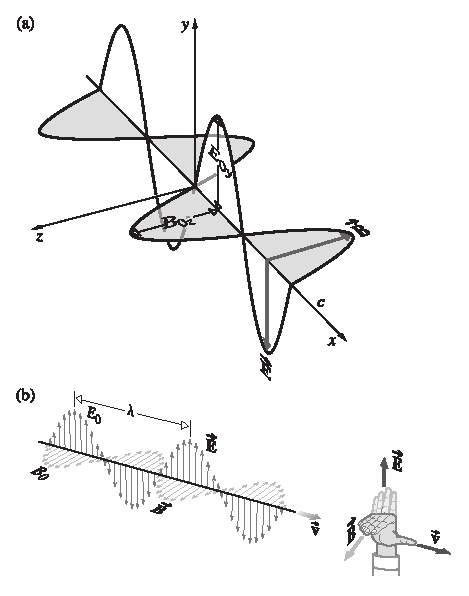
\includegraphics[width=0.75\linewidth]{Pictures/chap08/OrthogonalHarmonicPlaneEBField.eps}
    \caption{(a)平面偏振波中正交的简谐电场与磁场;(b)波在$\vec{\mathbf{E}}\times\vec{\mathbf{B}}$方向上传播。}
    \label{fig:08ex02.0314}
\end{figure}
一般的介电质材料是不导电和非磁性的,此时\refeq{08ex02-EycBz}可推广为
\begin{align}\label{eq:08ex02-EvB}
    E=vB\, ,
\end{align}
其中$\displaystyle v=\frac{1}{\sqrt{\epsilon\mu}}$是波在介质中的传播速度。
此外应注意,平面波并不是麦克斯韦方程组的唯一解,也有许多其他形式的解。

\subsubsection*{坡印廷矢量}
既然电磁波都存在于空间中,我们自然要考虑它单位体积内的辐射能,即能量密度$u$.
这意味着我们认为电磁场能存储能量,赋予了它实实在在的物理属性。
我们依然在经典的连续场框架下讨论该问题。

从\refeq{08ex02-ParallelEnergy},我们知道了电容为$C$的理想平行板电容器被充电到电压$U$时,
其电荷因相互作用而分布在电场中的能量。设平行板面积为$A$,板间距离为$d$,
结合平行板电容器的电容计算\refeq{08ex02-capacitanceParallel},可得板间单位体积的能量为
\begin{align}
    u_E=\frac{\displaystyle\frac{1}{2}CU^2}{Ad}=\frac{\displaystyle\frac{\epsilon_0 A}{2d}(Ed)^2}{Ad}=\frac{\epsilon_0}{2}E^2\, .
\end{align}

类似地,考虑电流为$I$电感为$L$的理想空心螺线管中的磁场,
设螺线管截面面积为$A$,长度为$l$,单位长度上绕线有$n$匝,则其电感为
\begin{align}
    L=\mu_0n^2lA\, ,
\end{align}
线圈内磁感应强度为
\begin{align}
    B=\mu_0nI\, ,
\end{align}
于是该区域内的能量密度为
\begin{align}
    u_B=\frac{\displaystyle\frac{1}{2}LI^2}{Al}=\frac{\displaystyle\frac{1}{2}\mu_0n^2lA\left(\frac{B}{\mu_0n}\right)^2}{Al}=\frac{1}{2\mu_0}B^2\, .
\end{align}
注意到\refeq{08ex02-EvB}可推广到适用于各种电磁波,取速度为光速$c$,联立\refeq{08ex02-speedOfLight}得到
\begin{align}
    u_E=u_B\, ,
\end{align}
这意味着,以电磁波形式流过空间的能量,由构成该电磁波的电场和磁场等量分享,
所以总能量密度为
\begin{align}
    u=u_E+u_B=\epsilon_0 E^2=\frac{1}{\mu_0}B^2\, .
\end{align}

注意场和$u$都是随时间变化的。我们用$S$表示单位时间内
电磁波穿过单位面积输送的能量(功率),单位为$\text{W}/\text{m}^2$.
电磁波以速度$c$在很短时间间隔$\Delta t$内穿过面积$A$,则有
\begin{align}
    S=\frac{uc\Delta tA}{\Delta tA}=uc=\frac{1}{\mu_0}EB=c^2\epsilon_0 EB\, .
\end{align}
我们(对各向同性介质)合理假设能量流动的方向就是波传播的方向,
由此定义\begin{marginfigure}
    \includegraphics[width=\linewidth]{chap08/JohnHenryPoynting.jpg}
\end{marginfigure}\sidenote{英国物理学家约翰·亨利·坡印廷 (John Henry Poynting, 1852-1914)。}\keyindex{坡印廷矢量}{Poynting vector}{vector\ 向量}
$\vec{\mathbf{S}}$为
\begin{align}
    \vec{\mathbf{S}}=c^2\epsilon_0\vec{\mathbf{E}}\times\vec{\mathbf{B}}\, ,
\end{align}
$\vec{\mathbf{S}}$的大小是穿过与$\vec{\mathbf{S}}$垂直的表面单位面积的功率。
例如,对于一个在方向$\vec{\mathbf{k}}$上穿过自由空间的线偏振(即电场和磁场方向固定)简谐平面波:
\begin{align}
    \vec{\mathbf{E}} & =\vec{\mathbf{E}}_0\cos(\vec{\mathbf{k}}\cdot\vec{\mathbf{r}}-\omega t)\, , \\
    \vec{\mathbf{B}} & =\vec{\mathbf{B}}_0\cos(\vec{\mathbf{k}}\cdot\vec{\mathbf{r}}-\omega t)\, ,
\end{align}
其坡印廷矢量为
\begin{align}
    \vec{\mathbf{S}}=c^2\epsilon_0\vec{\mathbf{E}}_0\times\vec{\mathbf{B}}_0\cos^2(\vec{\mathbf{k}}\cdot\vec{\mathbf{r}}-\omega t)\, .
\end{align}
它表示了单位时间内穿过单位面积的能量瞬时流动。
考虑到光的频率很大,$\vec{\mathbf{S}}$的变化是极快的,难以直接测量。
实践中我们更常使用其均值。记某函数$f(t)$在时间区间$T$上的均值为
\begin{align}
    \langle f(t)\rangle_T=\frac{1}{T}\int_{t-\frac{T}{2}}^{t+\frac{T}{2}}f(t')\mathrm{d}t'\, .
\end{align}
则对于上例有
\begin{align}
    \langle S\rangle_T=c^2\epsilon_0|\vec{\mathbf{E}}_0\times\vec{\mathbf{B}}_0|\langle\cos^2(\vec{\mathbf{k}}\cdot\vec{\mathbf{r}}-\omega t)\rangle_T\, .
\end{align}
考虑到在$T\gg t$时,$\langle\cos^2(\vec{\mathbf{k}}\cdot\vec{\mathbf{r}}-\omega t)\rangle_T=\displaystyle\frac{1}{2}$,
于是有
\begin{align}
    \langle S\rangle_T=\frac{c\epsilon_0}{2}E_0^2=\epsilon_0c\langle E^2\rangle_T=\frac{c}{\mu_0}\langle B^2\rangle_T\, .
\end{align}
它就是定义\ref{definition:05ex01-irradiance}中介绍的\keyindex{辐射通量密度}{radiant flux density}{},
按接收和发射分为辐射照度和辐射出射度。在线性均匀各向同性介电质中,上式可改写为
\begin{align}
    \langle S\rangle_T=\epsilon v\langle E^2\rangle_T\, ,
\end{align}
它表明辐射照度或辐射出射度与电场振幅的平方$E_0$成正比。

\subsubsection*{光子}
1900年普朗克\begin{marginfigure}
    \includegraphics[width=\linewidth]{chap08/MaxPlanckbyHugoErfurth1938.jpg}
\end{marginfigure}\sidenote{德国物理学家马克斯·卡尔·恩斯特·路德维希·普朗克 (Max Karl Ernst Ludwig Planck, 1858-1947)。}
在分析\keyindex{黑体辐射}{blackbody radiation}{}
过程时,为了解释观察到的现象,提出绝热室空腔的器壁上排列着振子,
振子只能以分立的能量份额吸收或发射能量(量子化),该份额与振子的振动频率$\nu$成正比,
且是$h\nu$的整数倍。这里物理常数$h$称作\keyindex{普朗克常数}{Planck constant}{},
在国际单位制下定义为精确值\sidenote{该常数如今被用来定义国际单位制中的质量单位“千克”。}
\begin{align}
    h=6.62607015\times10^{-34}\text{J}\cdot\text{s}\, .
\end{align}

1905年,爱因斯坦\begin{marginfigure}
    \includegraphics[width=\linewidth]{chap08/AlbertEinstein1947.jpg}
\end{marginfigure}\sidenote{德国犹太裔瑞士和美国双国籍理论物理学家阿尔伯特·爱因斯坦 (Albert Einstein, 1879-1955)。}
在光电效应的理论工作中,一鸣惊人地提出:电磁场本身是量子化的!
组成电磁场的每个光子的能量为
\begin{align}
    \mathcal{E}=h\nu\, .
\end{align}
\keyindex{光子}{photon}{}
是稳定的不带电荷且质量为零的基本粒子,且只能以速度$c$存在。
1932年,苏联科学家Evgenii M. Brumberg和Sergei I. Vavilov通过实验证明了光的基本量子本性。

不像普通物体,光子无法被直接看见,我们是通过光子的生成和湮灭来认识它的。
光子属于\keyindex{玻色子}{boson}{}\begin{marginfigure}
    \includegraphics[width=\linewidth]{chap08/SatyenBose.jpg}
\end{marginfigure}\sidenote{印度物理学家萨特延德拉·纳特·玻色 (Satyendra Nath Bose, 1894-1974)。},
是\keyindex{自旋}{spin}{}
为1的粒子,其集群方式服从\keyindex{玻色-爱因斯坦统计}{Bose-Einstein statistics}{},
允许大量光子占据同一状态。但我们无法准确预言每个光子会在何时到达何处,
只能说光是在随机时刻随机位置上以断断续续的冲击交出能量的。
若一幅光的图像投射到幕布上,则其上任一位置测得(或算得)的辐照度
与该位置检测到一个光子的概率成正比。
对于准单色的光,我们以光束的辐射通量密度除以对应的光子能量$\mathcal{E}$
即可得到\keyindex{平均光子通量密度}{mean photon flux density}{},
即单位时间内通过单位面积的平均光子数目。
户外光的量级约在$10^{16}\text{s}^{-1}\cdot\text{m}^{-2}$,
亮太阳光约$10^{18}\text{s}^{-1}\cdot\text{m}^{-2}$,
月光约$10^{12}\text{s}^{-1}\cdot\text{m}^{-2}$.

\subsubsection*{辐射压强和动量}
1873年麦克斯韦在理论上重新提出了对辐射压强的研究。
一束电磁波射到实物表面时,与组成大块实物的电荷相互作用,
对这些电荷从而对实物表面施加一个力,产生压强。
进一步地可以确定,电磁波本身具有\keyindex{动量}{momentum}{}。
麦克斯韦证明了,\keyindex{辐射压强}{radiation pressure}{}
$\mathcal{P}$等于电磁波的能量密度。
我们形式上对此进行简单说明:真空中,
考虑辐射能通量(功率)为$\varPhi$电磁波在时间$\Delta t$行进$\Delta x=c\Delta t$,
在面积$A$上等效施加的压力为$F$,做功为$\Delta W$,则结合坡印廷矢量的定义,辐射压强$\mathcal{P}$为
\begin{align}
    \mathcal{P}=\frac{F}{A}
    =\frac{\displaystyle\frac{F\Delta x}{\Delta t}}{A}\frac{\Delta t}{\Delta x}
    =\frac{\displaystyle\frac{\Delta W}{\Delta t}}{A}\frac{1}{c}=\frac{\varPhi}{Ac}=\frac{S}{c}=u\, .
\end{align}
所以我们可以将辐射压强用坡印廷矢量表示:
\begin{align}
    \mathcal{P}(t)=\frac{S(t)}{c}\, ,
\end{align}
这是垂直入射光施加在理想吸收面上的瞬时压强。
对应的平均辐射压强则为
\begin{align}
    \langle\mathcal{P}\rangle_T=\frac{\langle S(t)\rangle_T}{c}\, .
\end{align}
记电磁波动量的大小为$\Delta p$,则
\begin{align}
    \Delta p=F\Delta t=\mathcal{P}A\Delta t\, .
\end{align}
设$p_V$为单位体积辐射的动量,则
\begin{align}
    p_V=\frac{\Delta p}{Ac\Delta t}=\frac{\mathcal{P}}{c}=\frac{S}{c^2}\, .
\end{align}
推广到线性均匀各向同性介电质中,将动量的体积密度写成矢量形式,则有
\begin{align}
    \vec{\mathbf{p}}_V=\epsilon\vec{\mathbf{E}}\times\vec{\mathbf{B}}\, .
\end{align}

若被照射的是完全反射面,辐射以速度$+c$入射并以速度$-c$反射,则有
\begin{align}
    \langle\mathcal{P}\rangle_T=\frac{2\langle S(t)\rangle_T}{c}\, .
\end{align}

现在我们考虑单个光子的动量$p$.
设总动量$\Delta p$是由$N$个光子引发的。从能量角度,$N$应满足
\begin{align}
    N=\frac{\varPhi\Delta t}{\mathcal{E}}\, ,
\end{align}
于是单个光子的动量为
\begin{align}
    p=\frac{\Delta p}{N}=\frac{\mathcal{P}A\Delta t}{\displaystyle\frac{\varPhi\Delta t}{\mathcal{E}}}
    =\mathcal{P}\frac{A}{\varPhi}\mathcal{E}=\frac{S}{c}\frac{1}{S}\mathcal{E}
    =\frac{\mathcal{E}}{c}=\frac{h}{\lambda}\, .
\end{align}
其中$\lambda$为波长;对应的动量矢量为
\begin{align}
    \vec{\mathbf{p}}=\hslash\vec{\mathbf{k}}\, ,
\end{align}
其中$\vec{\mathbf{k}}$为传播向量,
$\hslash$为\keyindex{约化普朗克常数}{reduced Planck constant}{}
\begin{align}
    \hslash=\frac{h}{2\pi}\, .
\end{align}
狭义相对论把一个粒子的静止质量$m_0$、能量$\mathcal{E}$和动量$p$联系起来:
\begin{align}
    \mathcal{E}^2=(pc)^2+(m_0c^2)^2\, ,
\end{align}
对于光子$m_0=0$,有$\mathcal{E}=pc$,前面的结果与狭义相对论符合得很好。
这些量子力学观点已经被1923年实验中的\keyindex{康普顿效应}{Compton effect}{}
证实\begin{marginfigure}
    \includegraphics[width=\linewidth]{chap08/ArthurCompton1927.jpg}
\end{marginfigure}\sidenote{美国物理学家阿瑟·霍利·康普顿 (Arthur Holly Compton, 1892-1962)。}
——单个X射线光子与电子相互作用时将能量转给了电子并发生频移,且总动量守恒。

太阳垂直入射到紧贴地球大气层的面上的平均辐射照度约为$1400\text{W}/\text{m}^2$,
若被完全吸收,则产生的压强约$4.7\times10^{-6}\text{N}/\text{m}^2$,
对整个地球的压力总共约为10吨。这与大气压强约$10^5\text{N}/\text{m}^2$相比几乎可以忽略不计。
早在1901年,光压就被俄国实验物理学家彼得·尼古拉耶维奇·列别捷夫
(Pyotr Nikolaevich Lebedev, 1866-1912)测量到了。

\subsubsection*{电偶极子与电极化}
宏观物质置于电场中时,构成它的微观粒子会在电场作用下发生运动产生位移,
这种现象称为\keyindex{极化}{polarization}{}。
这些带电粒子分布的变化又会重新影响物质内部的电场分布。
因此在讨论电场对物质的作用时应考虑极化的影响。

电极化的有多种产生机制。在称为\keyindex{介电质}{dielectric}{}
的一大类绝缘材料中,电子被紧密束缚在\keyindex{原子核}{nucleus}{}
附近。虽然电子不能随意挪走,但在电场作用下,
带负电的电子云会相对于带正电的原子核产生微小位移与形变(如\reffig{08ex02-electronCloud}),
于是材料发生\keyindex{电子极化}{electronic polarization}{polarization\ 极化}。

此外,在\keyindex{极性分子}{polar molecule}{molecule\ 分子}
材料中,\keyindex{分子}{molecule}{}
的各原子不均等地分享\keyindex{价电子}{valence electron}{electron\ 电子},
所以正负电荷中心是永久分离的(\reffig{08ex02-moleculesDipole}),
在电场作用下,这种分子会因正负电荷受力方向相反而被牵拉朝着外加电场方向发生偏转,
发生\keyindex{取向极化}{orientational polarization}{polarization\ 极化}。

还一种情况是,对于NaCl那样的离子晶体,外加电场会使其正负离子发生相对位移,
发生\keyindex{离子极化}{ionic polarization}{polarization\ 极化},
也称\keyindex{原子极化}{atomic polarization}{polarization\ 极化}。
另外,还有非均质材料的结构界面阻挡带电粒子在外加电场下迁移而在分界面上累积电荷发生的\keyindex{界面极化}{interfacial polarization}{polarization\ 极化}
等其他情况。

这些电极化机制之间并不排斥,它们的综合效应带来了总的极化现象:
尽管材料整体呈电中性,但正负电荷轻微的分离产生了\keyindex{电偶极子}{electric dipole}{},
哪怕每个电偶极子含有等量的正负电荷,
其分布的不均衡也会累积出可观的净\keyindex{极化电荷}{polarization charge}{electric charge\ 电荷},
成为\keyindex{自由电荷}{free charge}{electric charge\ 电荷}
外又一电场来源。
\begin{figure}[htbp]
    \centering
    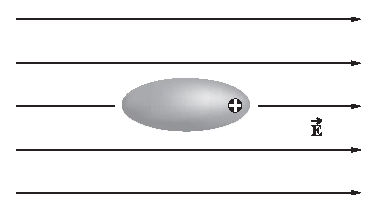
\includegraphics[width=0.5\linewidth]{chap08/electronCloud.eps}
    \caption{电场作用下的电子云发生微小位移与形变。}
    \label{fig:08ex02-electronCloud}
\end{figure}

最简单的电偶极子模型是一正一负含等量电荷$q$的分离点电荷,
记从负电荷指向正电荷的相对位移矢量为$\vec{\mathbf{d}}$.
我们定义该电偶极子的\keyindex{偶极矩}{dipole moment}{}
为
\begin{align}
    \vec{\mathbf{\srcp}}=q\vec{\mathbf{d}}\, .
\end{align}
其单位为$\text{C}\cdot\text{m}$.
对于更复杂的电偶极子,上述定义可推广为:
若电偶极子在区域$V$内关于位置矢量$\vec{\mathbf{r}}$的电荷分布体密度为$\rho(\vec{\mathbf{r}})$,
则其相应偶极矩为
\begin{align}
    \vec{\mathbf{\srcp}}=\iiint\limits_V\rho(\vec{\mathbf{r}})\vec{\mathbf{r}}\mathrm{d}V\, .
\end{align}
可以证明当电偶极子整体呈电中性时,其偶极矩具有平移不变性。
\begin{prove}
    把电偶极子原来整体所在位置设为原点,设其分布区域为$V$,
    然后平移到新位置$\vec{\mathbf{r}}_0$处,对应分布区域$V'$,则平移后的偶极矩为
    \begin{align}
        \vec{\mathbf{\srcp}}'
         & =\iiint\limits_{V'}\rho(\vec{\mathbf{r}}-\vec{\mathbf{r}}_0)\vec{\mathbf{r}}\mathrm{d}V'
        =\iiint\limits_{V'}\rho(\vec{\mathbf{r}}-\vec{\mathbf{r}}_0)(\vec{\mathbf{r}}-\vec{\mathbf{r}}_0+\vec{\mathbf{r}}_0)\mathrm{d}V'\nonumber \\
         & =\iiint\limits_{V'}\rho(\vec{\mathbf{r}}-\vec{\mathbf{r}}_0)(\vec{\mathbf{r}}-\vec{\mathbf{r}}_0)\mathrm{d}V'
        +\iiint\limits_{V'}\rho(\vec{\mathbf{r}}-\vec{\mathbf{r}}_0)\vec{\mathbf{r}}_0\mathrm{d}V'\nonumber                                       \\
         & =\iiint\limits_V\rho(\vec{\mathbf{r}})\vec{\mathbf{r}}\mathrm{d}V
        +\vec{\mathbf{r}}_0\iiint\limits_{V'}\rho(\vec{\mathbf{r}}-\vec{\mathbf{r}}_0)\mathrm{d}V'\nonumber                                       \\
         & =\vec{\mathbf{\srcp}}+\vec{\mathbf{r}}_0\cdot0\nonumber                                                                                \\
         & =\vec{\mathbf{\srcp}}\, .
    \end{align}
\end{prove}

\reffig{08ex02-moleculesDipole}展示了四种常见物质分子的偶极矩。
\begin{figure}[htbp]
    \centering
    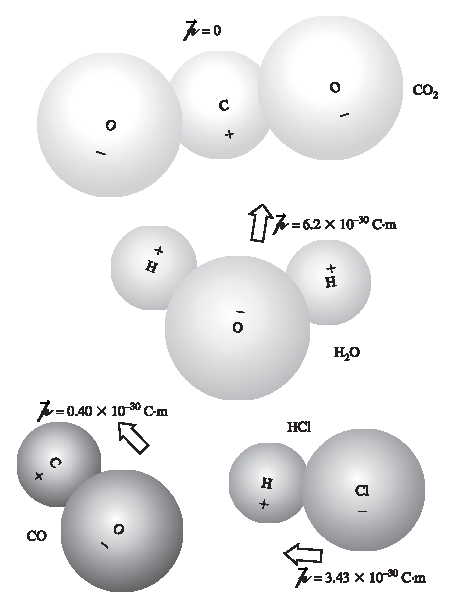
\includegraphics[width=0.8\linewidth]{chap08/moleculesDipole.eps}
    \caption{四种分子的偶极矩大小与方向,其中只有$\text{CO}_2$是非极性分子。}
    \label{fig:08ex02-moleculesDipole}
\end{figure}

接下来我们讨论最简电偶极子模型的电场和电势分布。
后面的推导中我们将经常用到以下两个关于矢量$\vec{\mathbf{r}}$的常见恒等式,
其中$\hat{\mathbf{r}}$是$\vec{\mathbf{r}}$方向上的单位向量,读者可自行验证:
\begin{align}
    \vec{\nabla}|\vec{\mathbf{r}}|           & =\frac{\vec{\mathbf{r}}}{|\vec{\mathbf{r}}|}=\hat{\mathbf{r}}\, ,                                  \\
    \vec{\nabla}\frac{1}{|\vec{\mathbf{r}}|} & =-\frac{\vec{\mathbf{r}}}{|\vec{\mathbf{r}}|^3}=-\frac{\hat{\mathbf{r}}}{|\vec{\mathbf{r}}|^2}\, .
\end{align}
我们取模型中两个点电荷连线的中点为原点,
并且正点电荷在$\displaystyle\frac{1}{2}\vec{\mathbf{d}}$处,
负点电荷在$-\displaystyle\frac{1}{2}\vec{\mathbf{d}}$处。
根据\refeq{08ex02-DistrubitionElectricPotential},
任意位置$\vec{\mathbf{r}}$处($r\gg d$)的电势为
\begin{align}
    \varphi(\vec{\mathbf{r}})=\frac{q}{4\pi\epsilon_0\left|\vec{\mathbf{r}}-\displaystyle\frac{1}{2}\vec{\mathbf{d}}\right|}
    +\frac{-q}{4\pi\epsilon_0\left|\vec{\mathbf{r}}-\left(-\displaystyle\frac{1}{2}\vec{\mathbf{d}}\right)\right|}\, .
\end{align}
考虑到$r\gg d$,我们只保留上式关于$d$的一次项,忽略高次项:
\begin{align}
    \varphi(\vec{\mathbf{r}})
     & =\frac{q}{4\pi\epsilon_0\left|\vec{\mathbf{r}}-\displaystyle\frac{1}{2}\vec{\mathbf{d}}\right|}
    -\frac{q}{4\pi\epsilon_0\left|\vec{\mathbf{r}}+\displaystyle\frac{1}{2}\vec{\mathbf{d}}\right|}\nonumber                            \\
     & \approx\frac{q}{4\pi\epsilon_0}\left(-\vec{\mathbf{d}}\cdot\vec{\nabla}\displaystyle\frac{1}{|\vec{\mathbf{r}}|}\right)\nonumber \\
     & =\frac{-q\vec{\mathbf{d}}}{4\pi\epsilon_0}\cdot\frac{-\hat{\mathbf{r}}}{|\vec{\mathbf{r}}|^2}\nonumber                           \\
     & =\frac{\vec{\mathbf{\srcp}}\cdot\hat{\mathbf{r}}}{4\pi\epsilon_0 r^2}\, ,
\end{align}
相应的电场为
\begin{align}
    \vec{\mathbf{E}}(\vec{\mathbf{r}})
     & =-\vec{\nabla}\varphi(\vec{\mathbf{r}})
    \approx-\vec{\nabla}\frac{\vec{\mathbf{\srcp}}\cdot\hat{\mathbf{r}}}{4\pi\epsilon_0 r^2}\nonumber                                                                              \\
     & =-\frac{1}{4\pi\epsilon_0}\vec{\nabla}\frac{\vec{\mathbf{\srcp}}\cdot\vec{\mathbf{r}}}{r^3}\nonumber                                                                        \\
     & =-\frac{1}{4\pi\epsilon_0 r^6}((\vec{\nabla}(\vec{\mathbf{\srcp}}\cdot\vec{\mathbf{r}}))\cdot r^3-(\vec{\mathbf{\srcp}}\cdot\vec{\mathbf{r}})\cdot\vec{\nabla}r^3)\nonumber \\
     & =-\frac{1}{4\pi\epsilon_0 r^6}(\vec{\mathbf{\srcp}}\cdot r^3-(\vec{\mathbf{\srcp}}\cdot\vec{\mathbf{r}})\cdot3r^2\cdot\frac{\vec{\mathbf{r}}}{|\vec{\mathbf{r}}|})\nonumber \\
     & =\frac{3(\vec{\mathbf{\srcp}}\cdot\hat{\mathbf{r}})\hat{\mathbf{r}}-\vec{\mathbf{\srcp}}}{4\pi\epsilon_0 r^3}\, .
\end{align}

\subsubsection*{电偶极辐射}
若一个电荷进行变速运动,它就会辐射。
在垂直于引起辐射的加速度方向上,辐射能量最强。
辐射的能量是某个外部动力对电荷做功使其变速运动而供给的。
最简单直观的电磁波产生机制是振荡的电偶极子,
它由一正一负两个电荷组成,沿直线做往复运动。
实物系统辐射能量虽然是量子力学过程,但可以用经典的振荡电偶极子来设想其能量发射速率。
\reffig{08ex02.0332}示意地画出了一个电偶极子的电场分布,
其中一个负电荷在一个静止且大小相等的正电荷旁做直线简谐运动。
若振动的角频率为$\omega$,则关于时间$t$的偶极矩有标量形式
\begin{align}
    \srcp(t)=\srcp_0\cos(\omega t)\, ,
\end{align}
这里$\srcp(t)$可以代表原子尺度上振荡电荷分布的总体偶极矩,
也甚至可以代表直线电视天线中的振荡电流。
如\reffig{08ex02.0332}(a),在$t=0$时,$\srcp=\srcp_0=qd$,
其中$d$是两个电荷中心间的初始最大间距。偶极矩实际上是一个向量,
方向是从$-q$指向$+q$;随着时间推移,偶极矩减小直到零然后反向,如此循环。
当两个电荷重合时,$\srcp=0$,电场线自身必定闭合。
\begin{figure}[htbp]
    \centering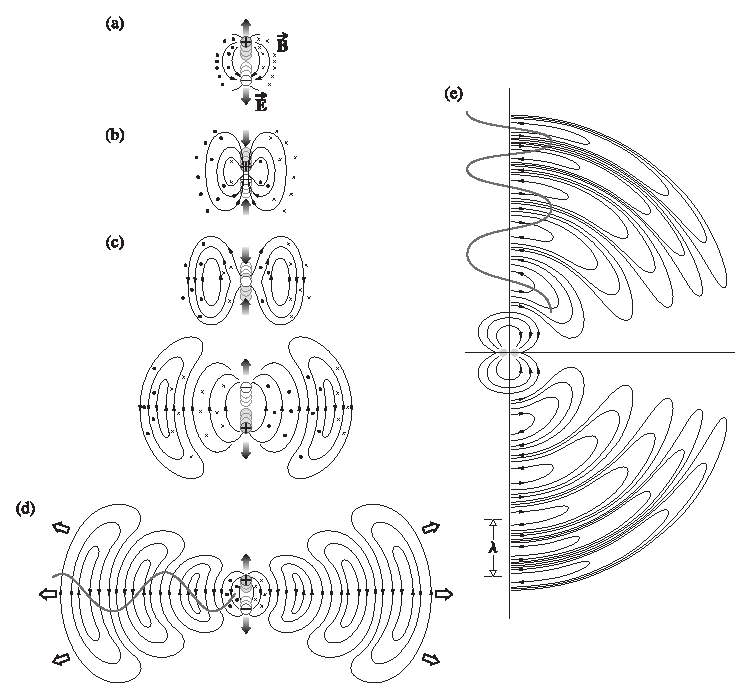
\includegraphics[width=\linewidth]{Pictures/chap08/OscillatingElectricDipole.eps}
    \caption{振荡的电偶极子的电场$\vec{\mathbf{E}}$.}
    \label{fig:08ex02.0332}
\end{figure}

在靠近偶极子的地方,电场的形状接近静止的电偶极子电场;
而在稍微远离的地方形成的闭环区域内,则没有明确的波长,其构成项非常复杂;
而更加远离的地方则称为波区或辐射区,那里场的构型则简单了许多,建立起固定的波长。
如\reffig{08ex02.0333},电场和磁场都是横波且相互正交同相,
磁力线是一些同心圆,圆心在偶极子轴上,圆所在平面垂直于偶极子轴。
坡印廷矢量则总是沿径向$\vec{\mathbf{r}}$向外。电场具体形式为
\begin{align}
    E=\frac{\srcp_0k^2\sin\theta\cos(kr-\omega t)}{4\pi\epsilon_0r}\, ,
\end{align}
其中$\theta$为径向与偶极子轴的夹角,从源向外的径向辐射的辐射照度为
\begin{align}
    \langle S\rangle_T(\theta)=\frac{\srcp_0^2\omega^4\sin^2\theta}{32\pi^2c^3\epsilon_0r^2}\, .
\end{align}
注意其中的$\omega^4$项,说明频率越高,辐射越强;而$r^2$项说明其对距离遵循平方反比定律。
\begin{figure}[htbp]
    \centering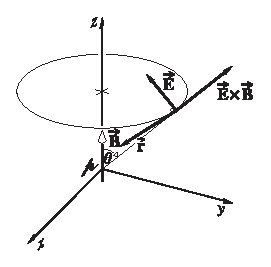
\includegraphics[width=0.4\linewidth]{Pictures/chap08/FieldOrientationsElectricDipole.eps}
    \caption{振荡的电偶极子中场的朝向。}
    \label{fig:08ex02.0333}
\end{figure}
